\chapter{Oracle Aplication Express}

\section{Tahapan Membuat Aplikasi Akademik Sederhana Oracle Apex}
Sebelum membuat aplikasi nya pertama harus menyiapkan data mentahan yang berasal dari materi Basis Data bab 3 Semester 1, kedua kita menormalisasi tabel-tabel yang ada pada bab 3 Basis Data Semester 1,yaitu Tabel Mahasiswa,Dosen,kuliah,Nilai,dan Jadwal.Untuk lebih pahamnya akan saya praktikan tahapan pembuatan Aplkasi pada Oracle Apex Online:  
\begin{enumerate}

\begin{figure}
\item[1.]Menormalisasi dan Membuat Tabel Mahasiswa di EXCEL. Dengan field NIM,Nama Mahasiswa,Alamat Mahasiswa,Tgl lahir.
    \begin{center}
    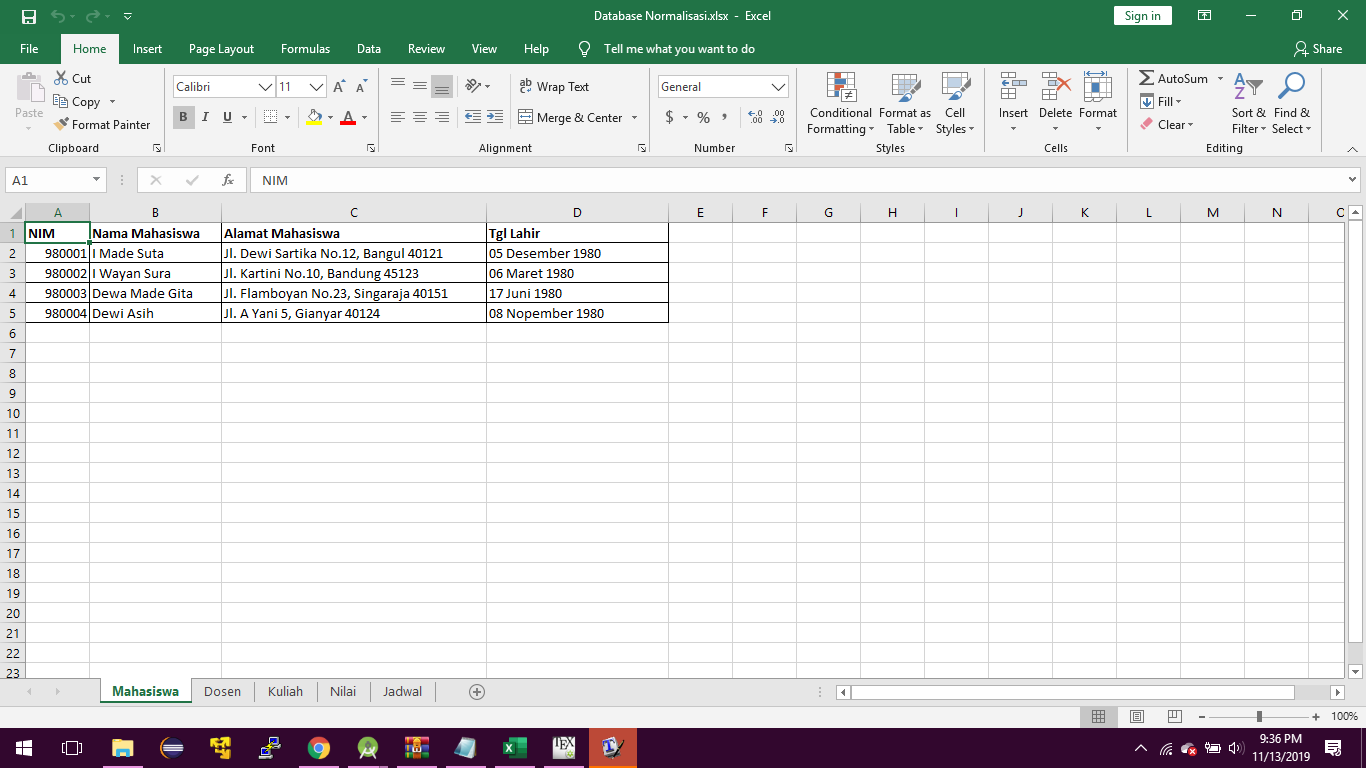
\includegraphics[scale=0.3]{figures/mhs.png}
    \caption{\textit{Tabel Mahasiswa.}}
    \end{center}   
    \end{figure}

\begin{figure}
\item[2.]Menormalisasi dan Membuat Tabel Dosen di ECXEL. Dengan Field NIK,Nama Dosen,Alamat Dosen.
    \begin{center}
    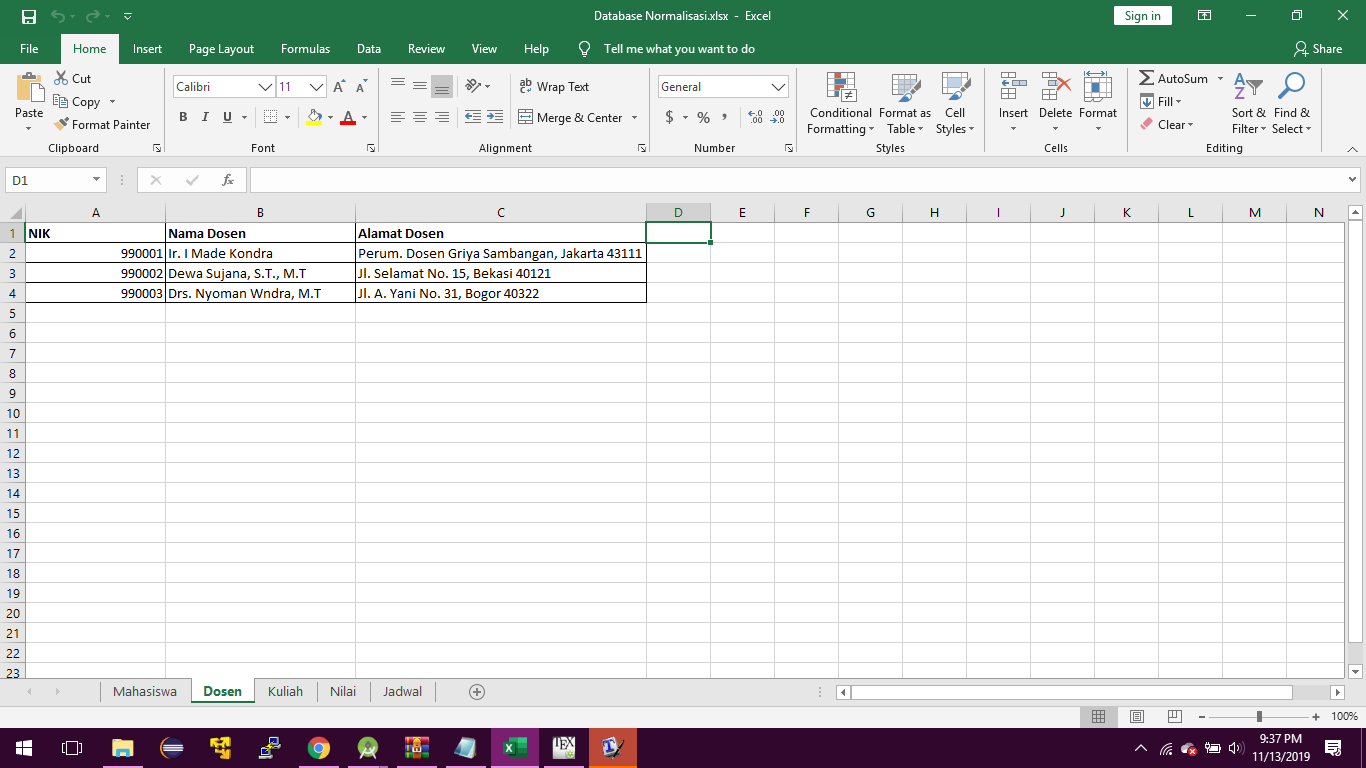
\includegraphics[scale=0.3]{figures/dosen.png}
    \caption{\textit{Tabel Dosen.}}
    \end{center}
    \label{gambar}
    \end{figure}

\begin{figure}
\item[3.]Menormalisasi dan Membuat Tabel Kuliah di ECXEL. Dengan Field Kode,SKS,Semester.
    \begin{center}
    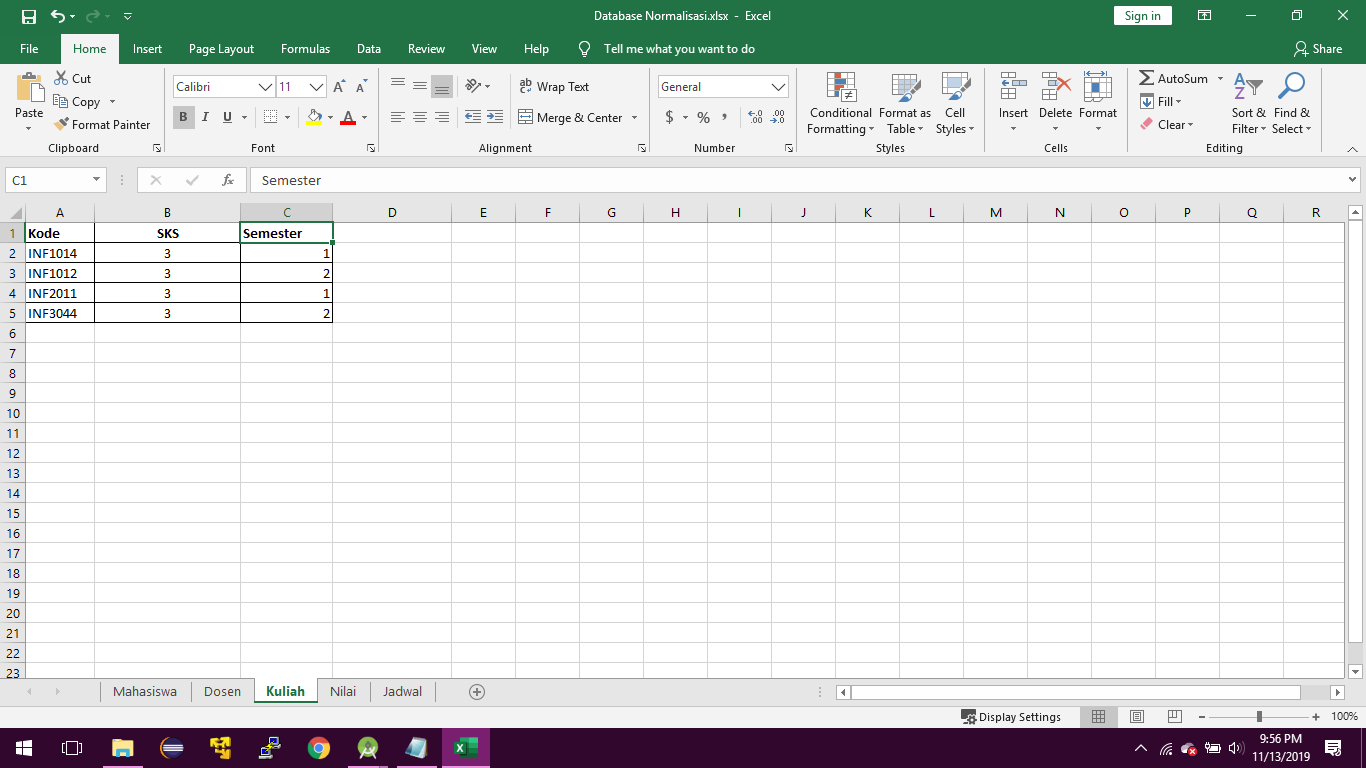
\includegraphics[scale=0.3]{figures/kuliah.png}
    \caption{\textit{Tabel Kuliah.}}
    \end{center}
    \label{gambar}
    \end{figure}

\begin{figure}
\item[4.]Menormalisasi dan Membuat Tabel Nilai di EXCEL. Dengan Field Kode,NIM,Indeks Nilai. 
    \begin{center}
    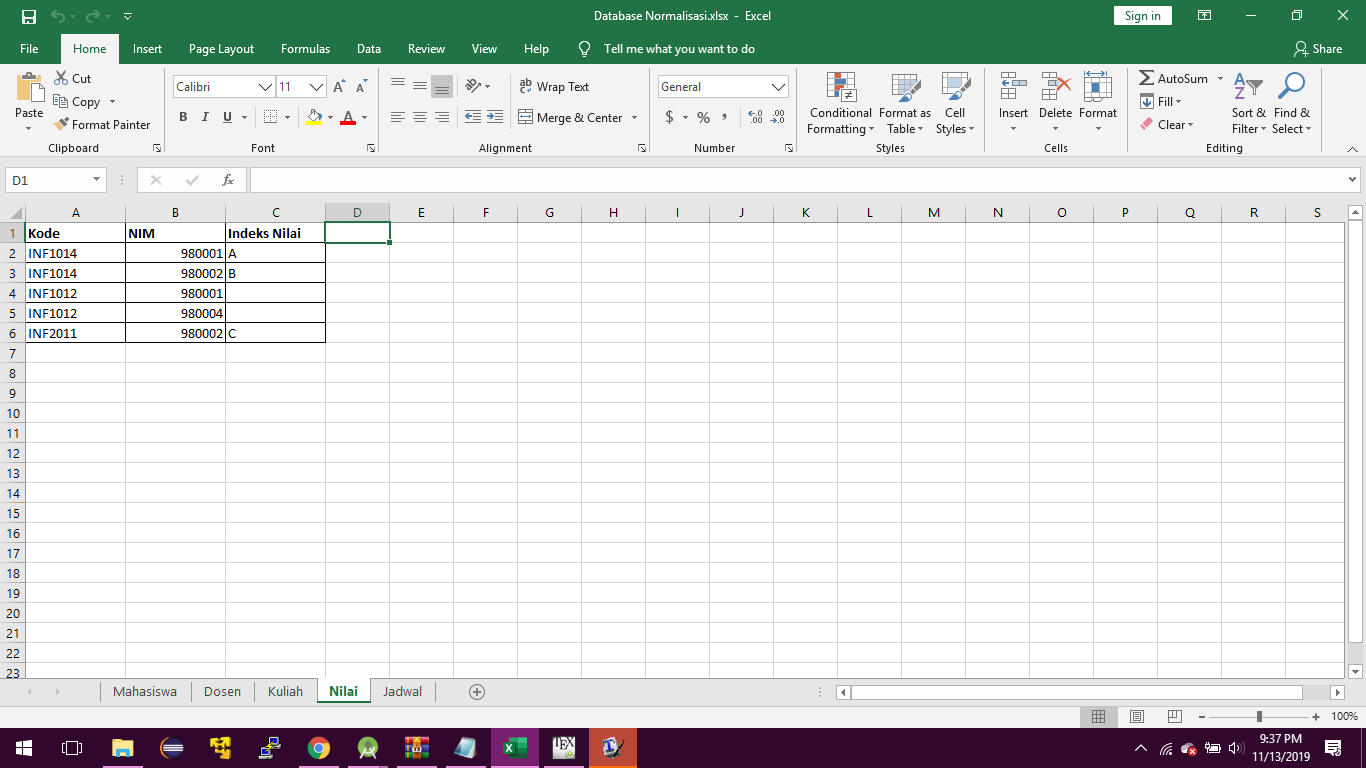
\includegraphics[scale=0.3]{figures/nilai.png}
    \caption{\textit{Tabel NIlai.}}
    \end{center}
    \label{gambar}
    \end{figure}

\begin{figure}
\item[5.]Menormalisasi dan Membuat Tabel Jadwal di EXCEL. Dengan Field Kode,NIK,Waktu,Tempat.
    \begin{center}
    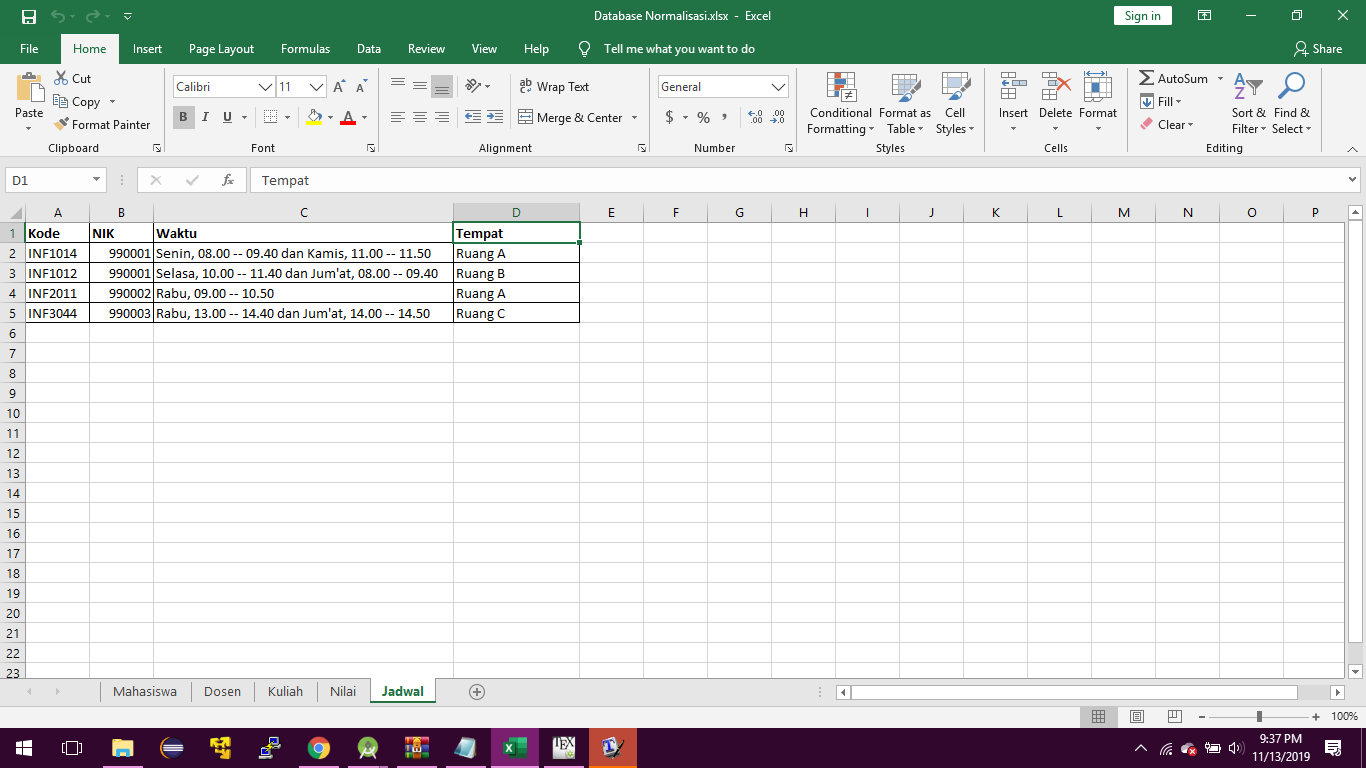
\includegraphics[scale=0.3]{figures/jadwal.png}
    \caption{\textit{Tabel Jadwal.}}
    \end{center}
    \label{gambar}
    \end{figure}

\begin{figure}
\item[6.] Setelah Tabel Selesai dibuat, Selanjutnya kita Login pada Aplikasi Oracle Apex Online. Dan jika belum memiliki akun pada oracle apex online utuk membuat akun terlebih dahulu pada get started for free lalu ikuti saja langkah-langkahnya.
    \begin{center}
    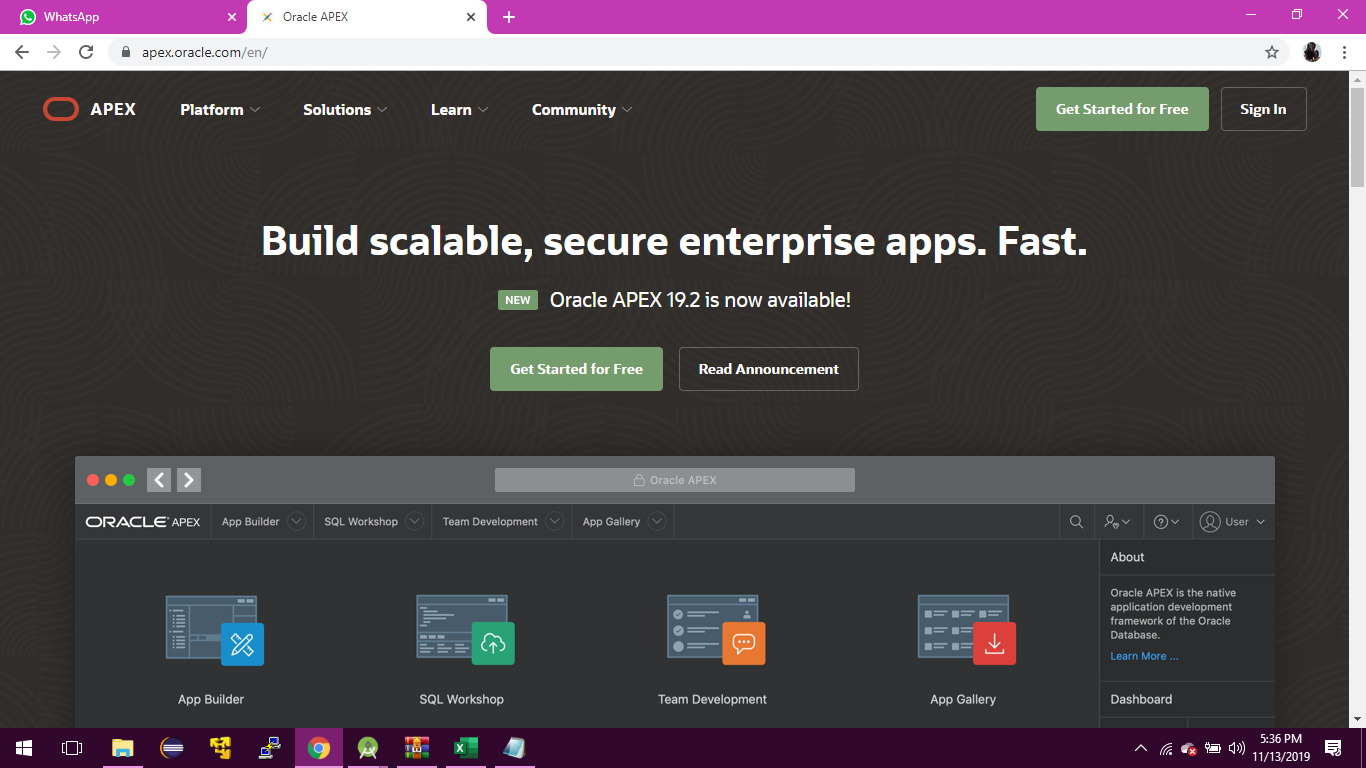
\includegraphics[scale=0.3]{figures/1.png}
    \caption{\textit{Tampilan daftar oracle apex online.}}
     \end{center}
    \label{gambar}
    \end{figure}

\begin{figure}
\item[7.]Jika sudah memiliki akun maka klik saja fitur sign in.Lalu akan muncul tampilan seperti di bawah dan isi workspace nya.
    \begin{center}
    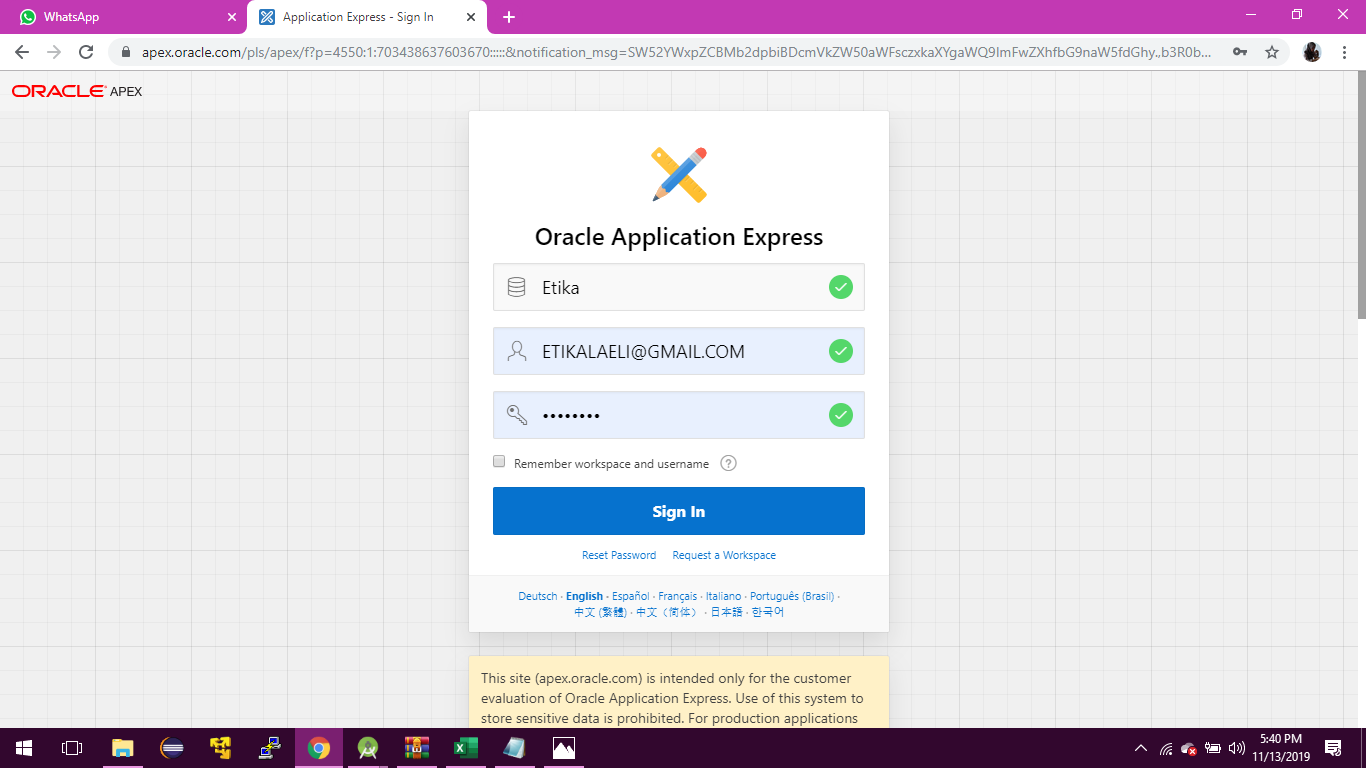
\includegraphics[scale=0.3]{figures/2.png}
    \caption{\textit{Login Aplikasi.}}
    \end{center}
    \label{gambar}
    \end{figure}

\begin{figure}
\item[8.]Pilih From app builder.
    \begin{center}
    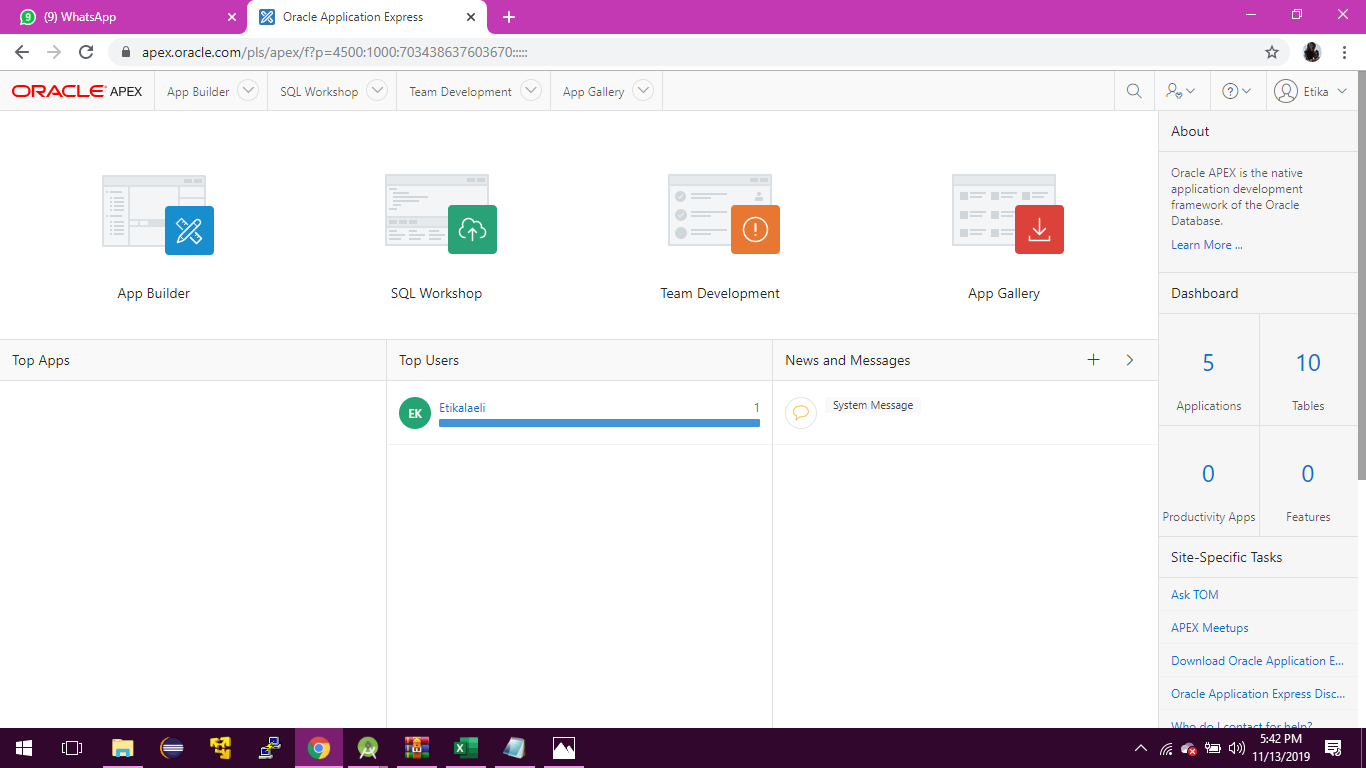
\includegraphics[scale=0.3]{figures/3.png}
    \caption{\textit{Pilih App Builder.}}
    \end{center}
    \label{gambar}
    \end{figure}
    
\begin{figure}
\item[9.]Kemudian pilih create.   
    \begin{center}
    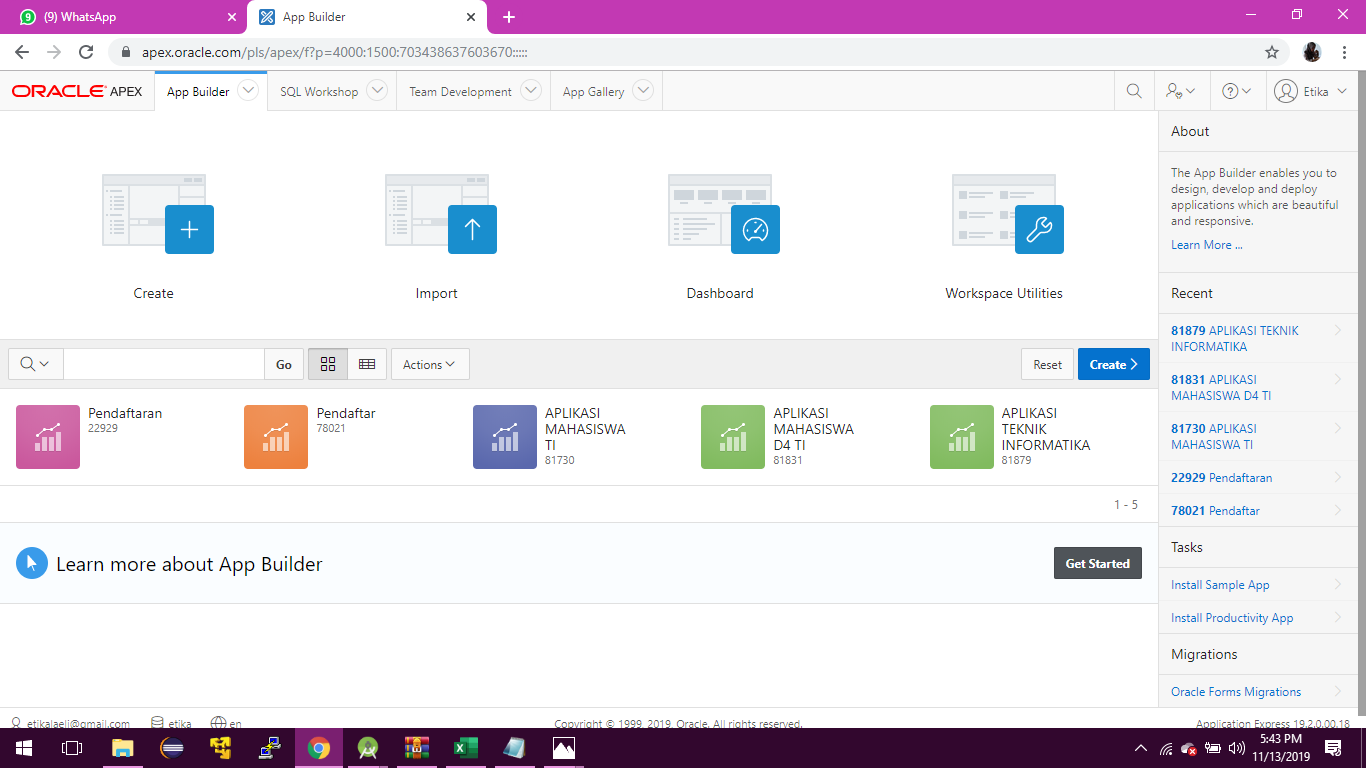
\includegraphics[scale=0.3]{figures/4.png}
    \caption{\textit{Pilih Create.}}
    \end{center}
    \label{gambar}
    \end{figure}

\begin{figure}
\item[10.]Setelah create, pilih from a file lalu chosee file yang tadi sudah di normalisasikan.
    \begin{center}
    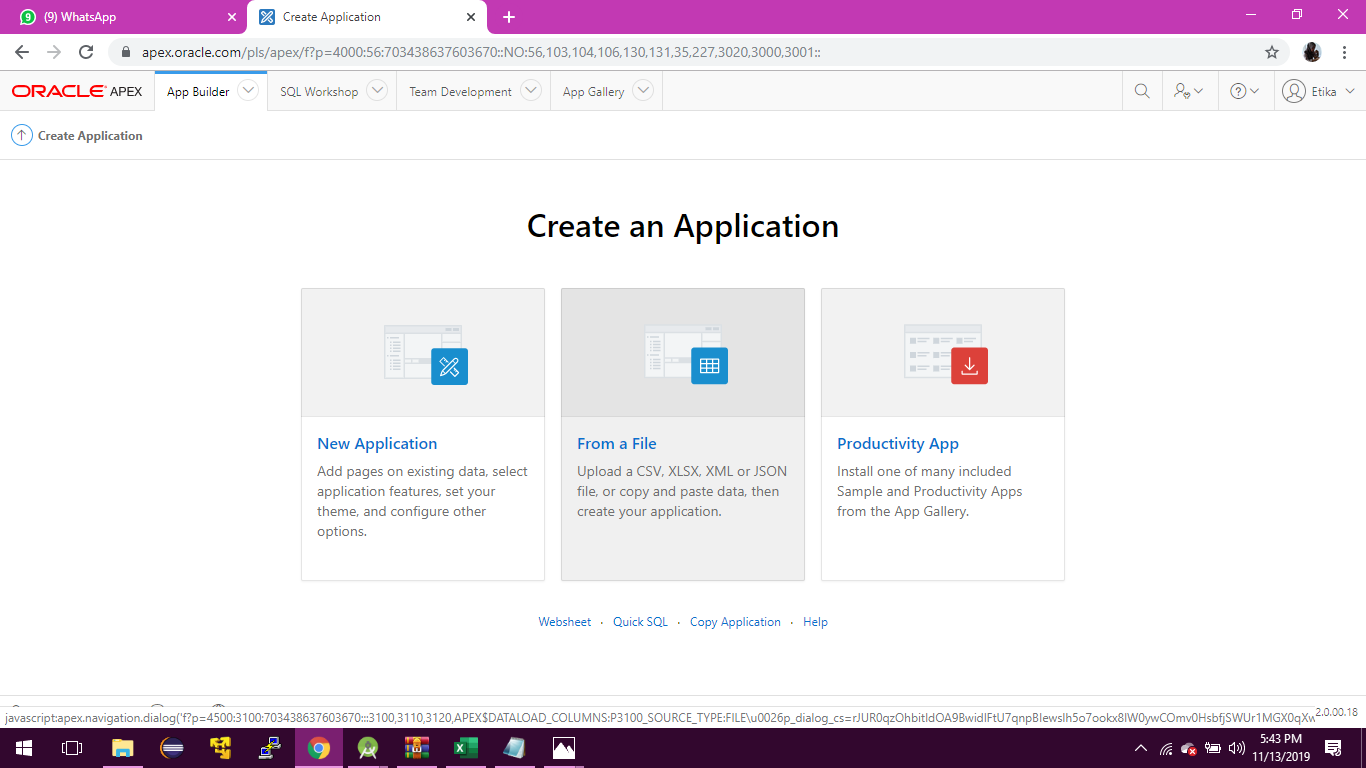
\includegraphics[scale=0.3]{figures/5.png}
    \caption{\textit{Pilih from a file.}}
     \end{center}
    \label{gambar}
    \end{figure}
 
\begin{figure}
\item[11.]Setelah create, pilih from a file lalu chosee file yang tadi sudah di normalisasikan.
    \begin{center}
    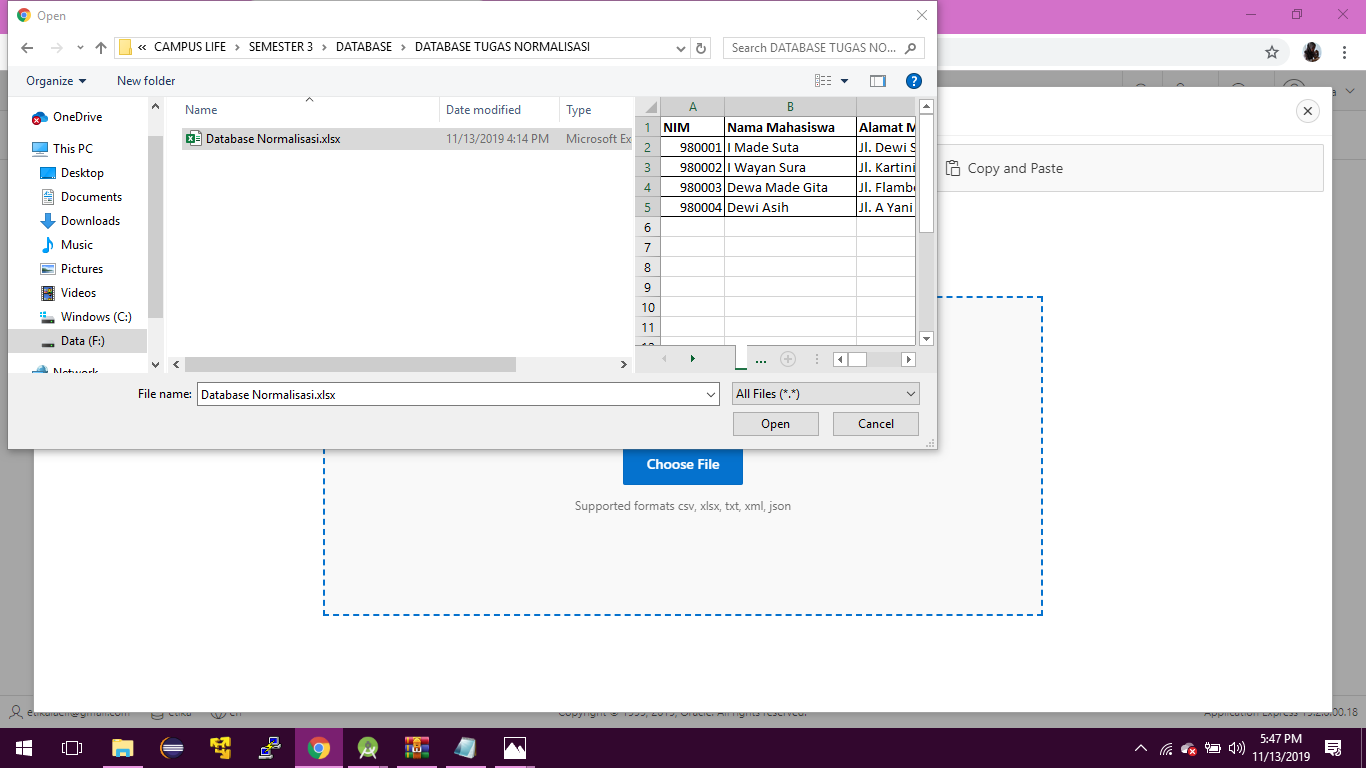
\includegraphics[scale=0.3]{figures/6.png}
    \caption{\textit{Masukan file.}}
     \end{center}
    \label{gambar}
    \end{figure}

\begin{figure}
\item[12.]Buat nama tabel sesuai dengan urutan yang telah dibuat pada file yang telah di normalisasikan tadi, dari yang tabel pertama sampe tabel terakhir, pertama yaitu tabel Mahasiswaa. Setelah selesai mengisinya lalu Load data.
    \begin{center}
    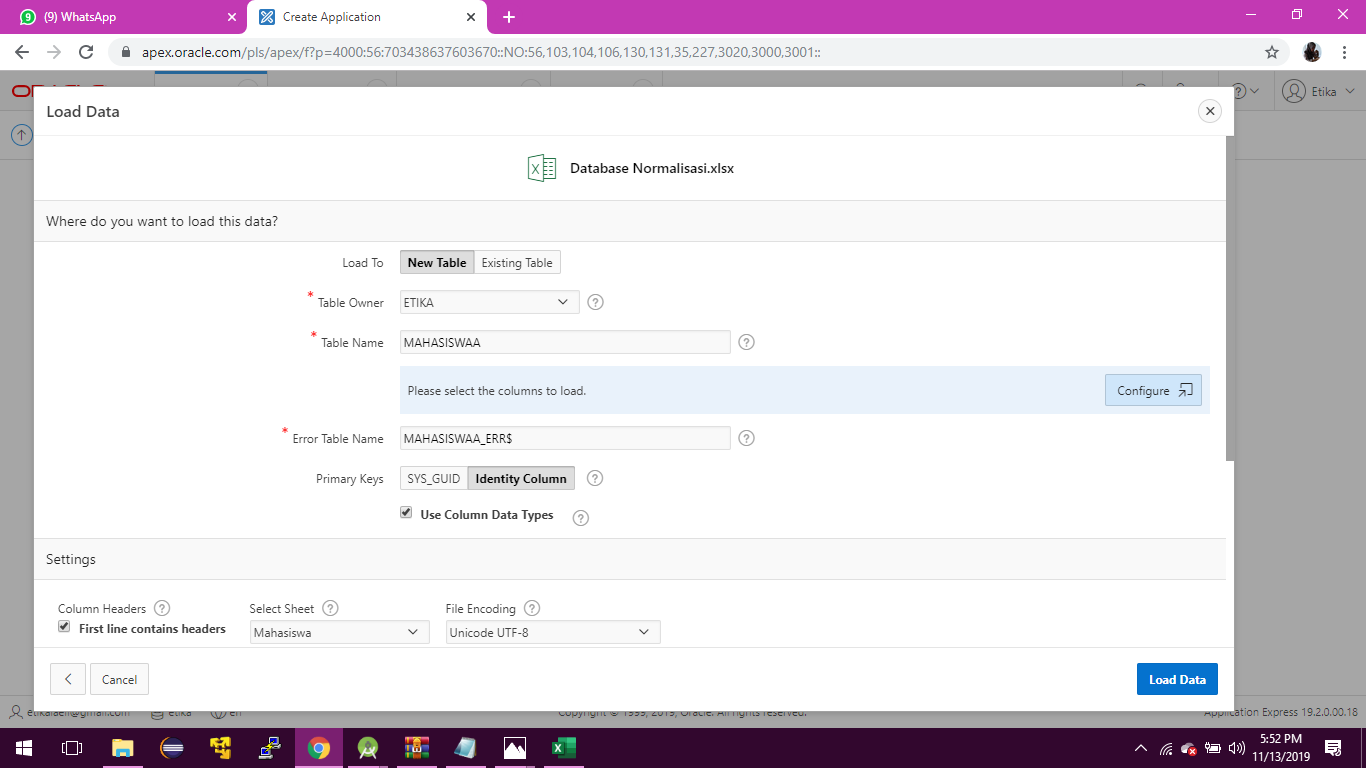
\includegraphics[scale=0.3]{figures/7.png}
    \caption{\textit{Beri nama Tabel Mahasiswaa.}}
    \end{center}
    \label{gambar}
    \end{figure}

\begin{figure}
\item[13.]Buat nama tabel sesuai dengan urutan yang telah dibuat pada file yang telah di normalisasikan tadi, dari yang tabel pertama sampe tabel terakhir,kedua yaitu tabel Dosen. Kemudian setelah selesai mengisinya lalu Load data.
    \begin{center}
    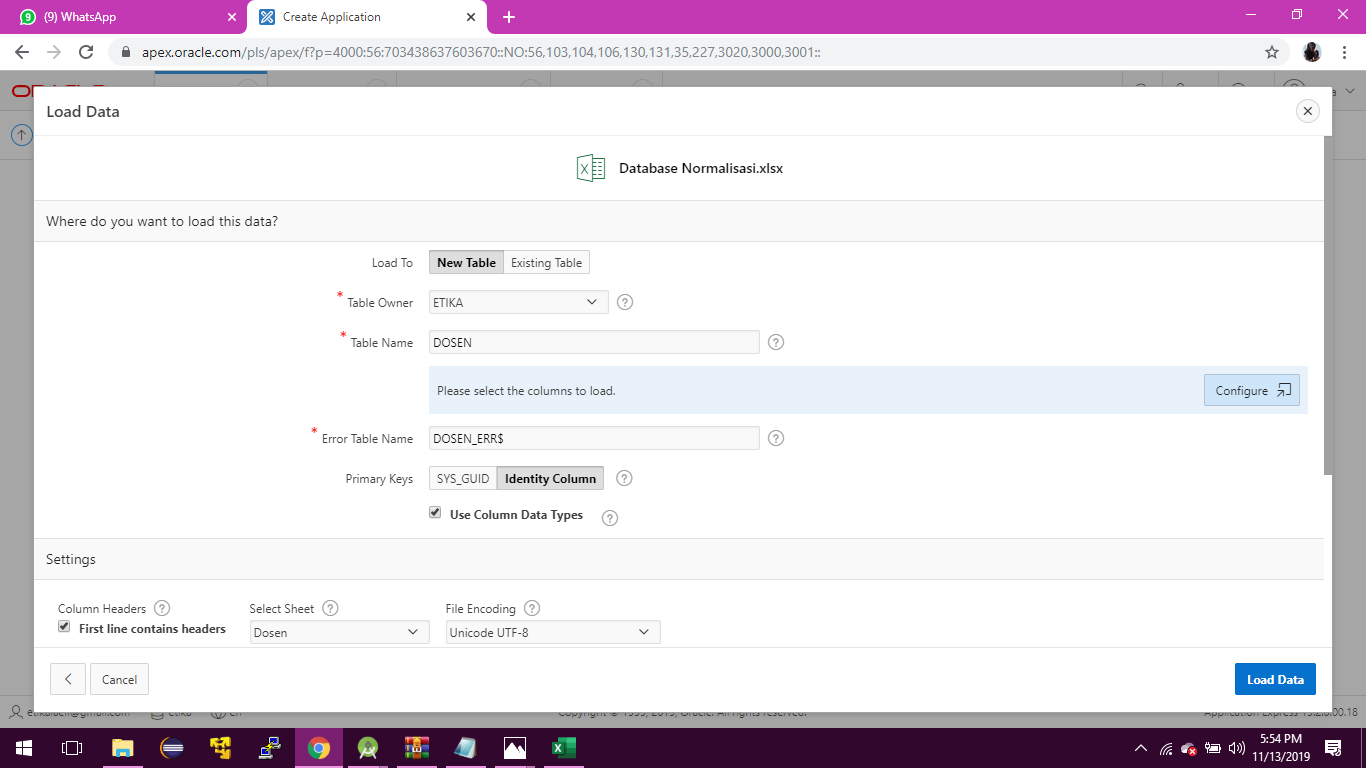
\includegraphics[scale=0.3]{figures/10.png}
    \caption{\textit{Beri nama Tabel Dosen.}}
    \end{center}
    \label{gambar}
    \end{figure}

\begin{figure}
\item[14.]Buat nama tabel sesuai dengan urutan yang telah dibuat pada file yang telah di normalisasikan tadi, dari yang tabel pertama sampe tabel terakhir, ketiga yaitu Tabel Kuliah kemudian setelah selesai mengisinya lalu Load data.
    \begin{center}
    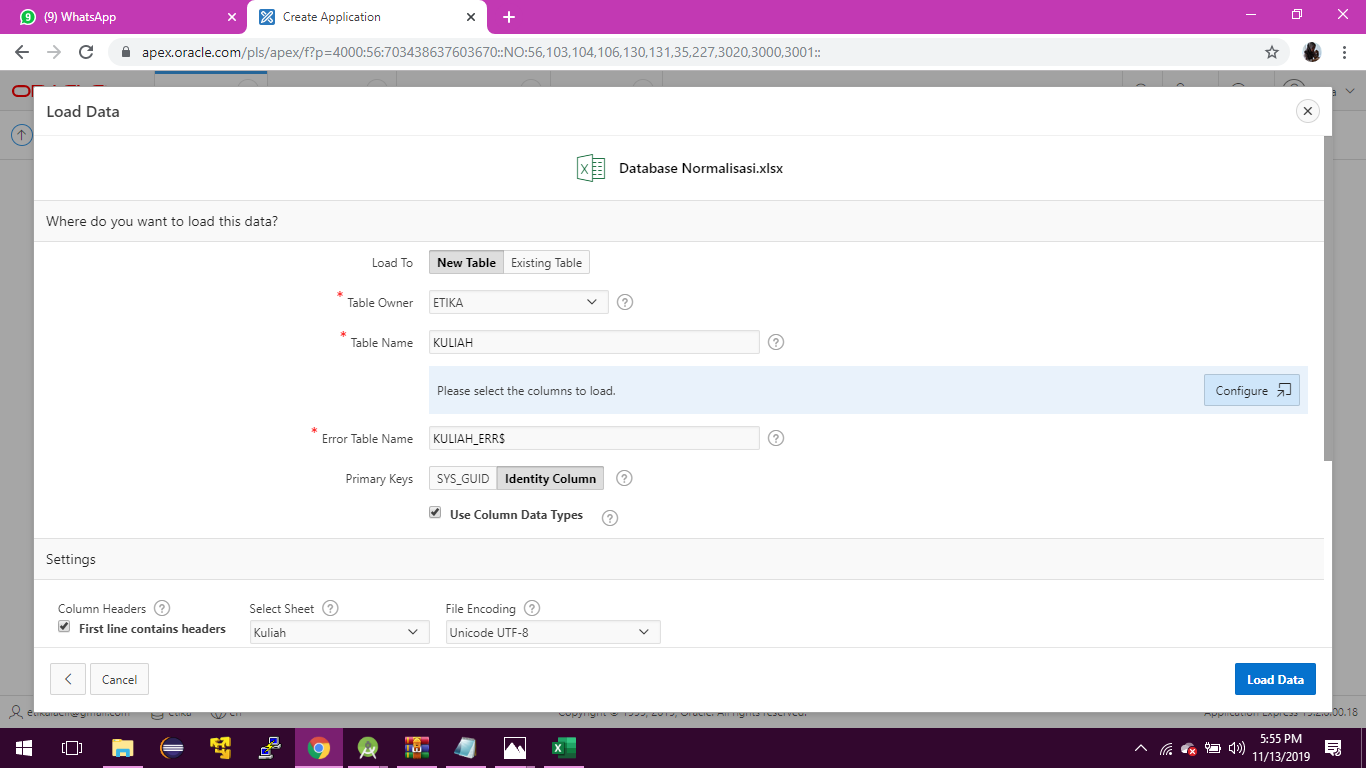
\includegraphics[scale=0.3]{figures/13.png}
    \caption{\textit{Beri nama Tabel Kuliah.}}
    \end{center}
    \label{gambar}
    \end{figure}

\begin{figure}
\item[15.]Buat nama tabel sesuai dengan urutan yang telah dibuat pada file yang telah di normalisasikan tadi, dari yang tabel pertama sampe tabel terakhir, keempat yaitu Tabel Nilai kemudian setelah selesai mengisinya lalu Load data.    
    \begin{center}
    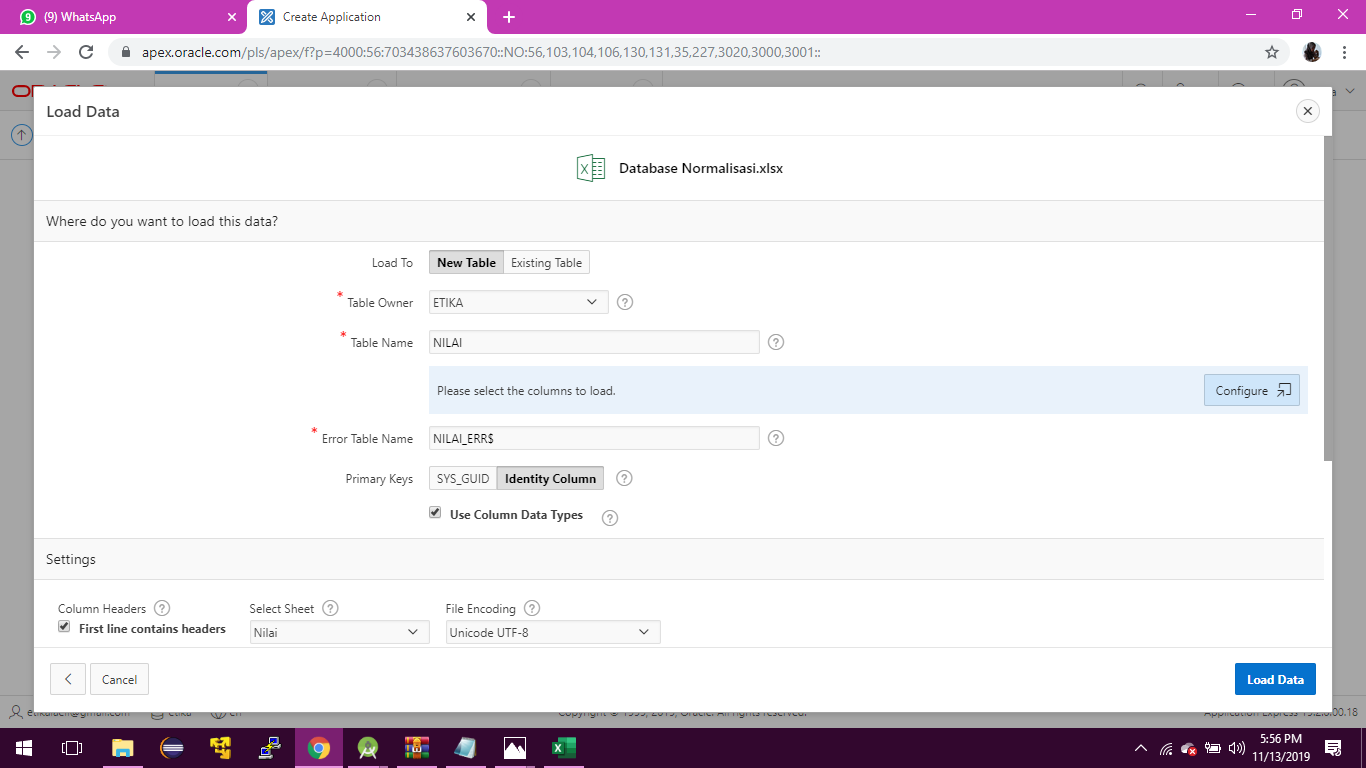
\includegraphics[scale=0.3]{figures/16.png}
    \caption{\textit{Beri nama Tabel Nilai.}}
    \end{center}
    \label{gambar}
    \end{figure}


\begin{figure}
\item[16.]Buat nama tabel sesuai dengan urutan yang telah dibuat pada file yang telah di normalisasikan tadi, dari yang tabel pertama sampe tabel terakhir yaitu Tabel Jadwal kemudian setelah selesai mengisinya lalu Load data. 
    \begin{center}
    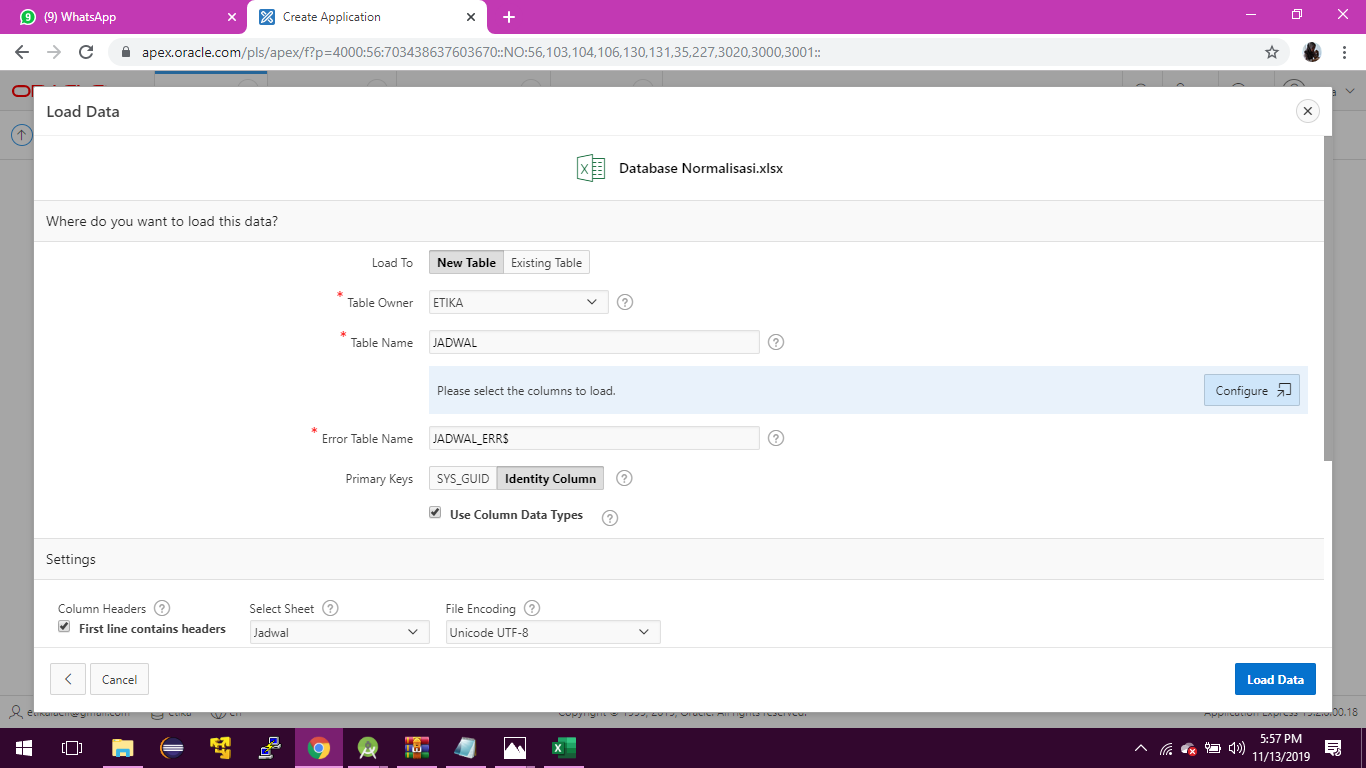
\includegraphics[scale=0.3]{figures/19.png}
    \caption{\textit{Beri nama Tabel Jadwal.}}
    \end{center}
    \label{gambar}
    \end{figure}

\begin{figure}
\item[17.]Tabel Telah Berhasil kita buat.
    \begin{center}
    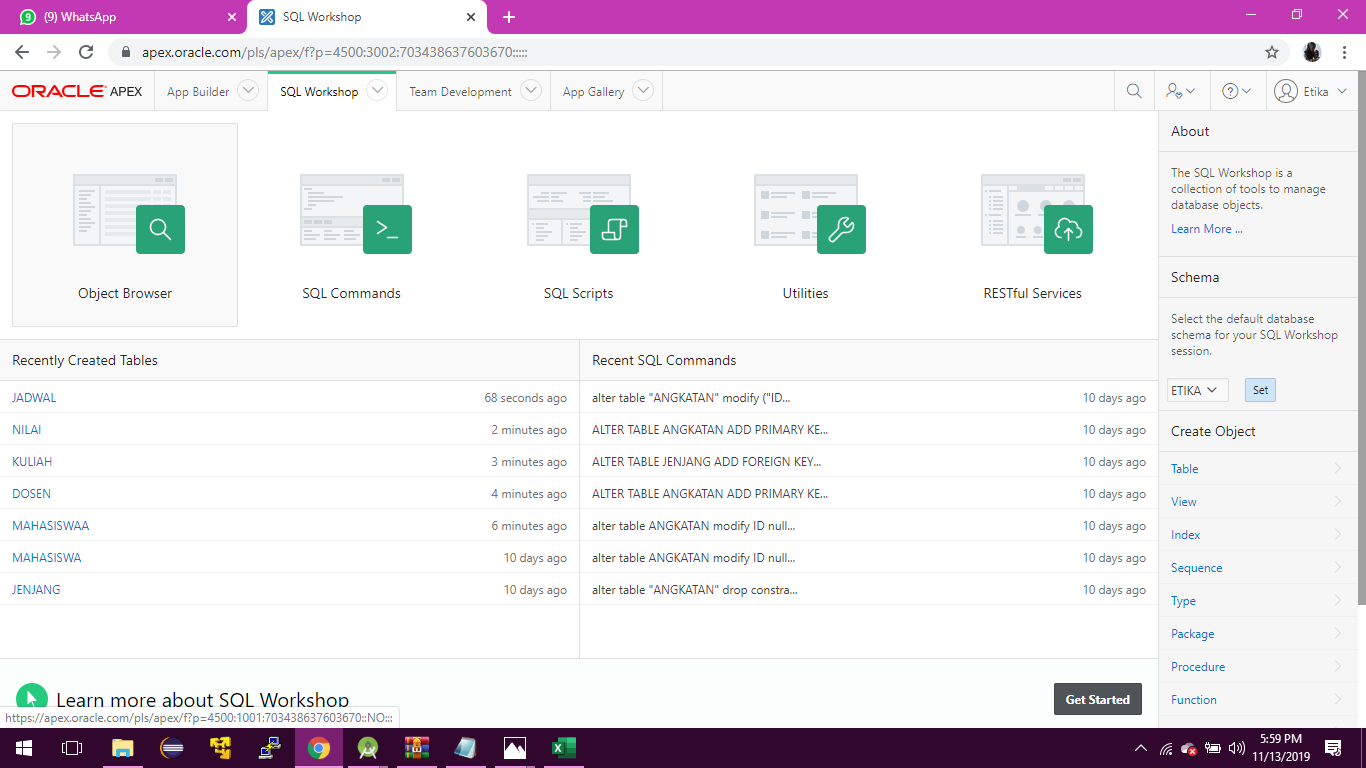
\includegraphics[scale=0.3]{figures/23.png}
    \caption{\textit{Tabel Berhasi Dibuat.}}
    \end{center}
    \label{gambar}
    \end{figure}

\begin{figure}
\item[18.]Masuk ke SQL Workshop, Pilih Object Browser, Lalu Hilangkan ID yang berada di semua tabel.Pertama tabel Mahasiswaa.
    \begin{center}
    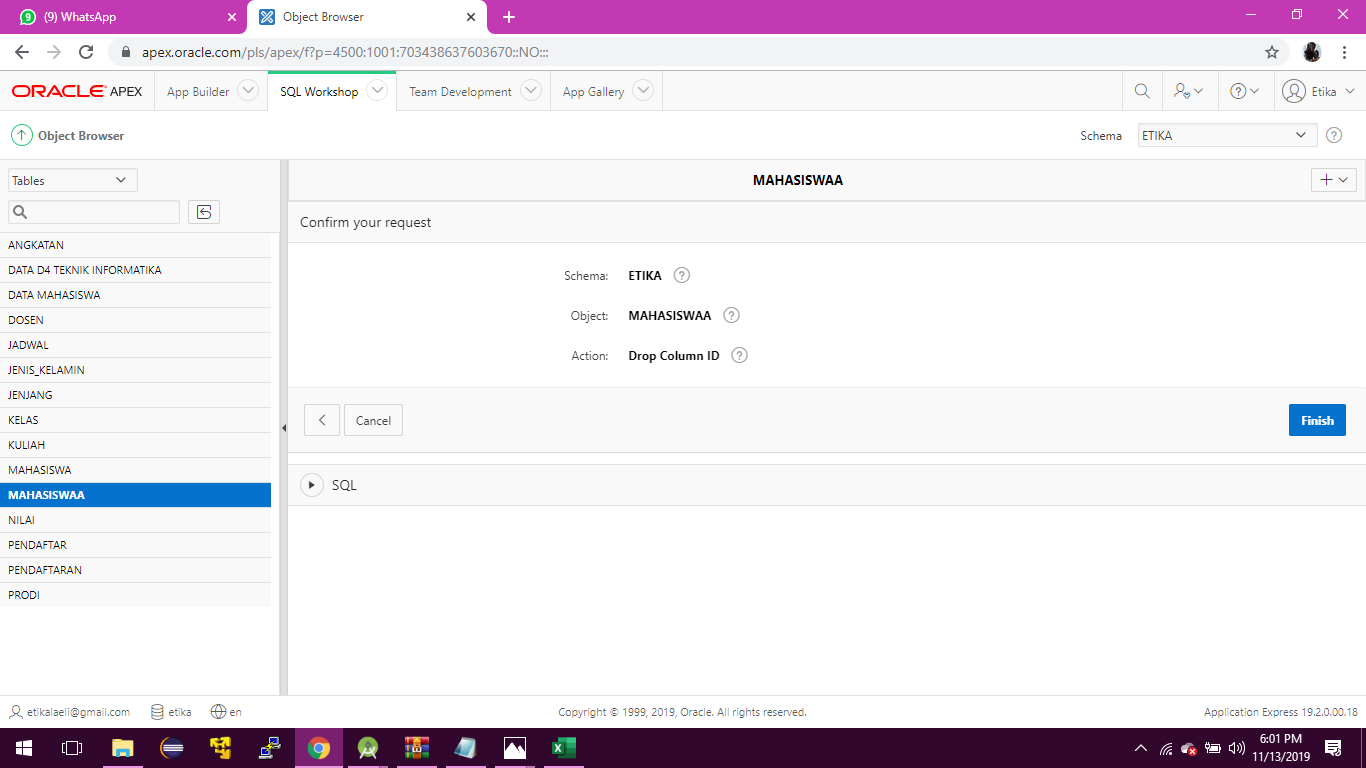
\includegraphics[scale=0.3]{figures/25.png}
    \caption{\textit{Hilangkan id Mahasiswa.}}
    \end{center}
    \label{gambar}
    \end{figure}

\begin{figure}
\item[19.]Masuk ke SQL Workshop, Pilih Object Browser, Lalu Hilangkan ID yang berada di semua tabel.Kedua tabel Dosen.   
    \begin{center}
    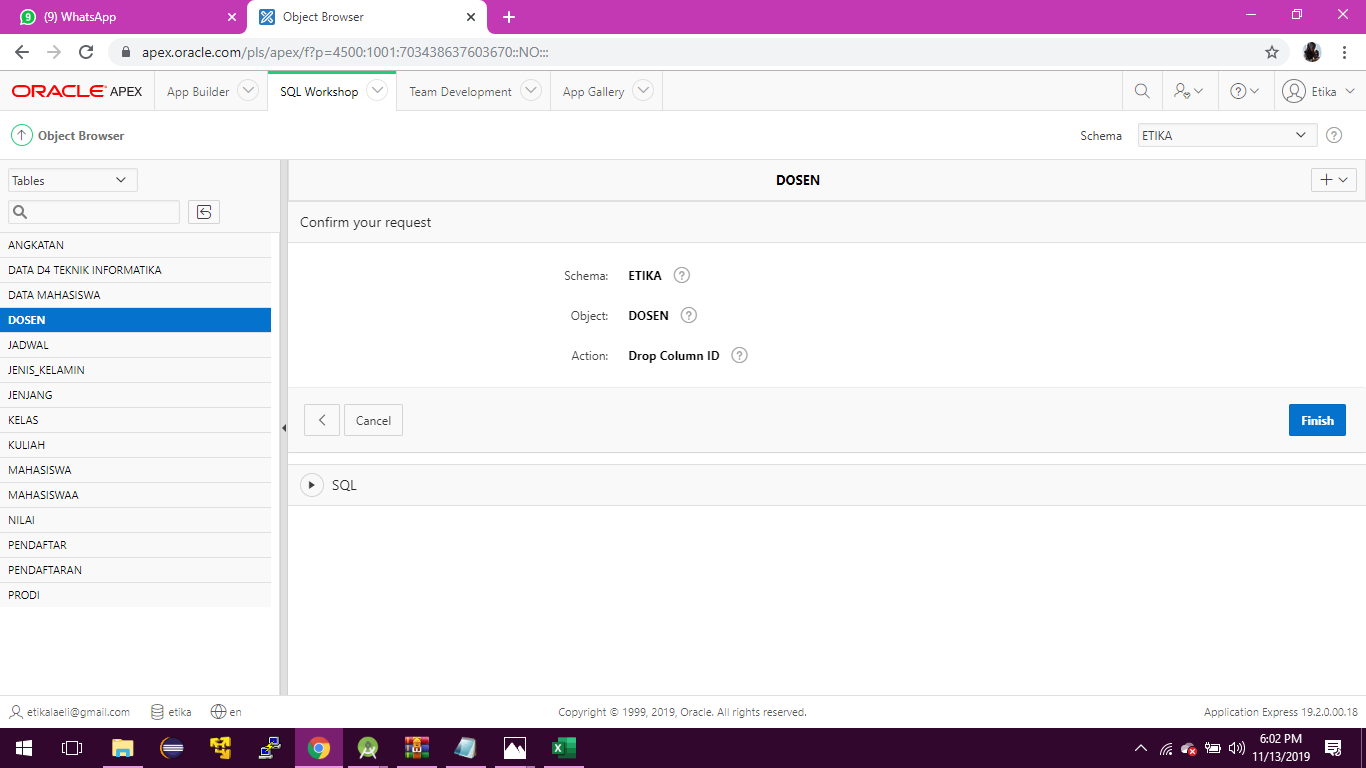
\includegraphics[scale=0.3]{figures/28.png}
    \caption{\textit{Hilangkan id Dosen.}}
    \end{center}
    \label{gambar}
    \end{figure}

\begin{figure}
\item[20.]Masuk ke SQL Workshop, Pilih Object Browser, Lalu Hilangkan ID yang berada di semua tabel.Ketiga tabel Kuliah.       
    \begin{center}
    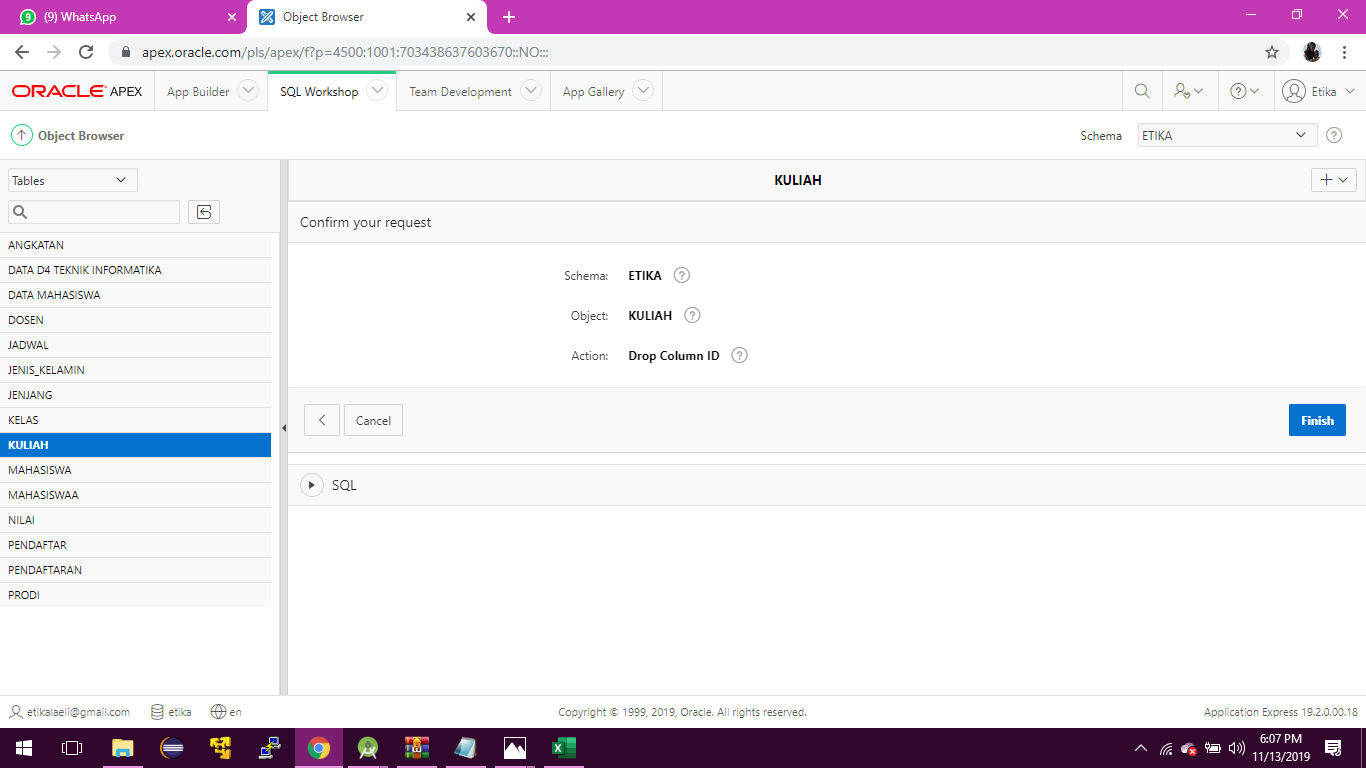
\includegraphics[scale=0.3]{figures/31.png}
    \caption{\textit{Hilangkan id Kuliah.}}
    \end{center}
    \label{gambar}
    \end{figure}

\begin{figure}
\item[21.]Masuk ke SQL Workshop, Pilih Object Browser, Lalu Hilangkan ID yang berada di semua tabel.Keempat tabel Nilai.        
    \begin{center}
    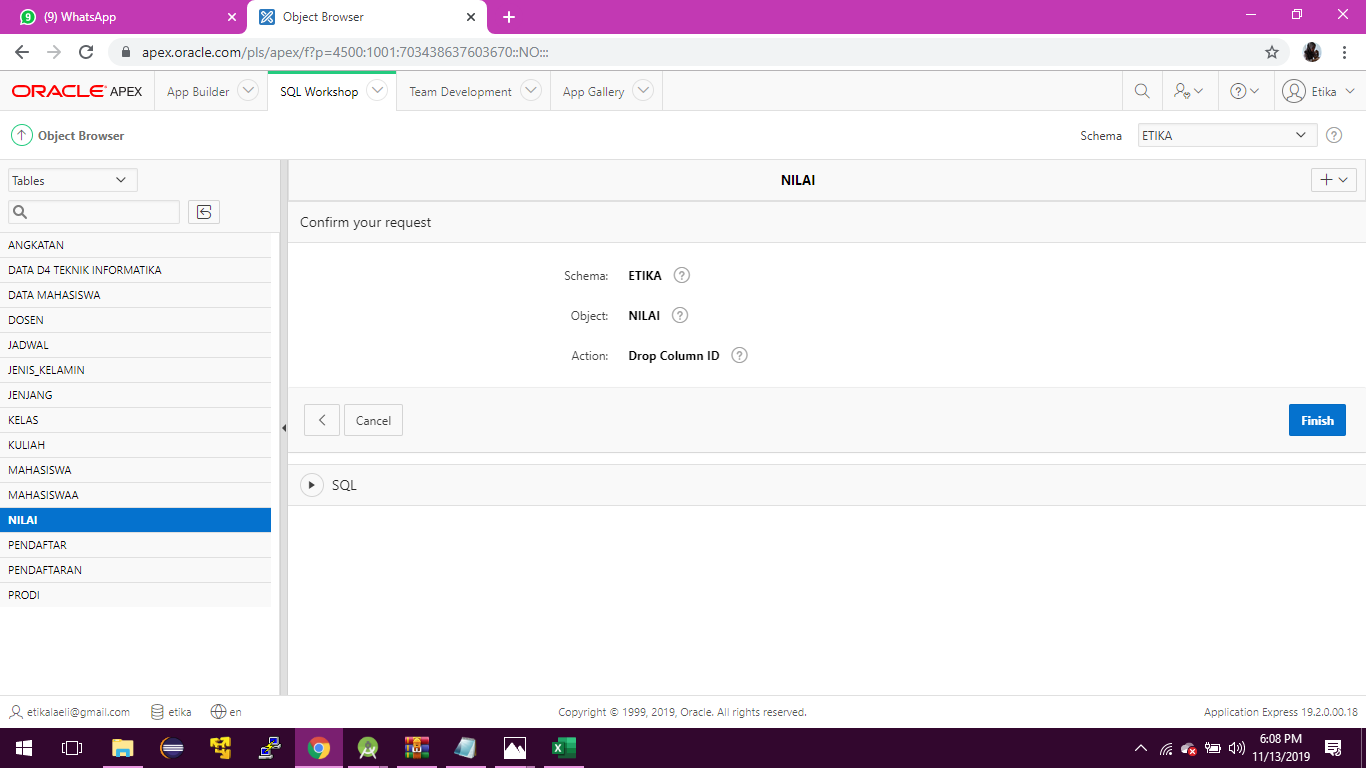
\includegraphics[scale=0.3]{figures/34.png}
    \caption{\textit{Hilangkan id Nilai.}}
    \end{center}
    \label{gambar}
    \end{figure}

\begin{figure}
\item[22.]Masuk ke SQL Workshop, Pilih Object Browser, Lalu Hilangkan ID yang berada di semua tabel. kelima tabel Jadwal.        
    \begin{center}
    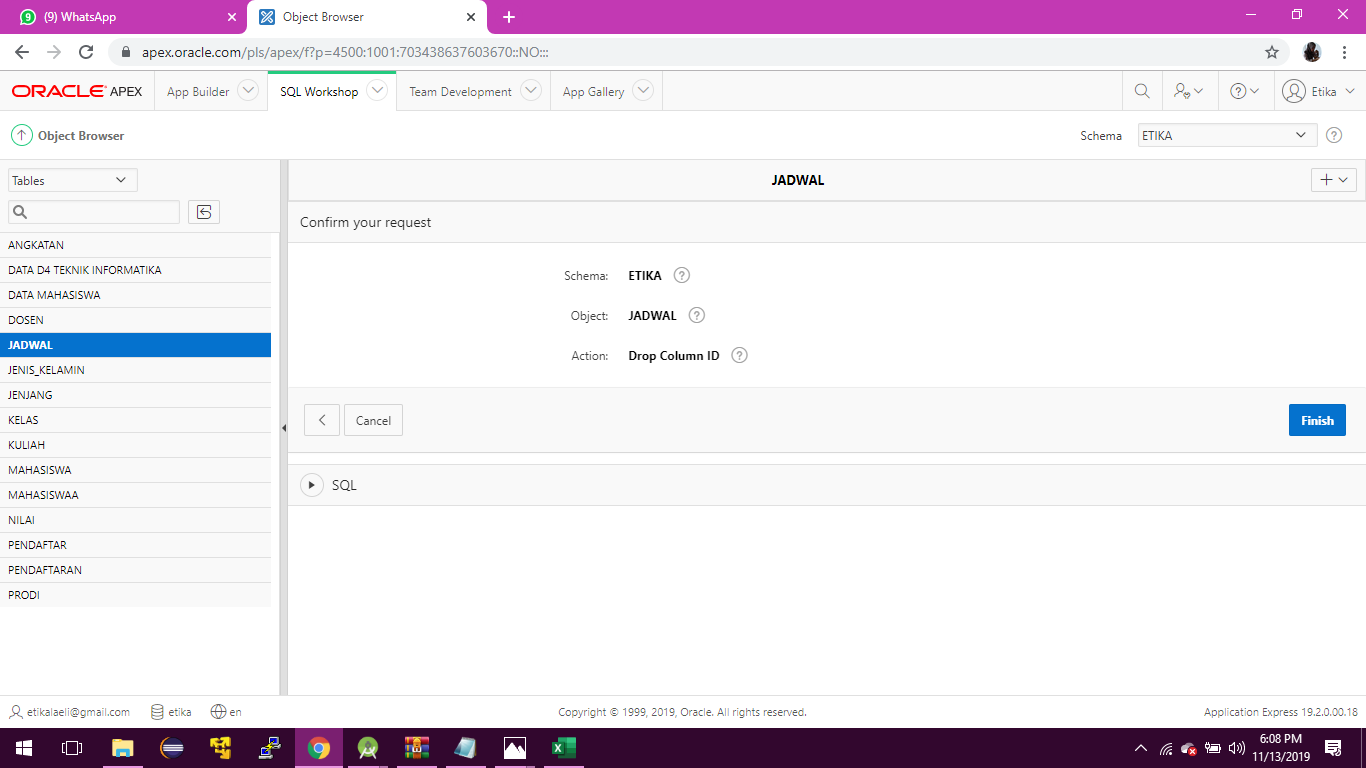
\includegraphics[scale=0.3]{figures/37.png}
    \caption{\textit{Hilangkan id Jadwal.}}
    \end{center}
    \label{gambar}
    \end{figure}
    
\begin{figure}
\item[23.]Pilih Tabel Mahasiswaa, Clik Constrains, create Jadikan NIM Sebagai Primary Key, Lalu Next. 
    \begin{center}
    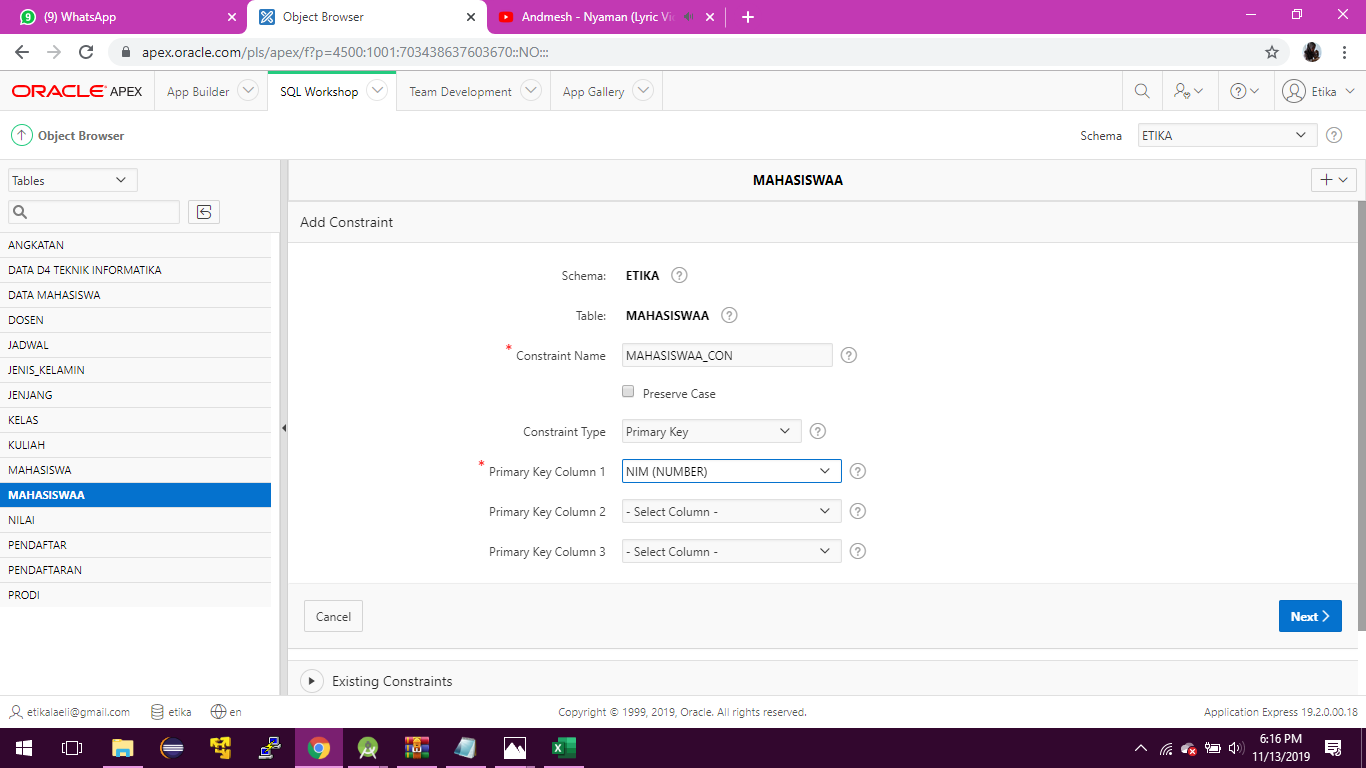
\includegraphics[scale=0.3]{figures/45.png}
    \caption{\textit{Tabel Mahasiswa.}}
    \end{center}
    \label{gambar}
    \end{figure}
    
\begin{figure}
\item[24.]Pilih Tabel Dosen, Clik Constrains, create Jadikan NIK Sebagai Primary Key, Lalu Next. 
    \begin{center}
    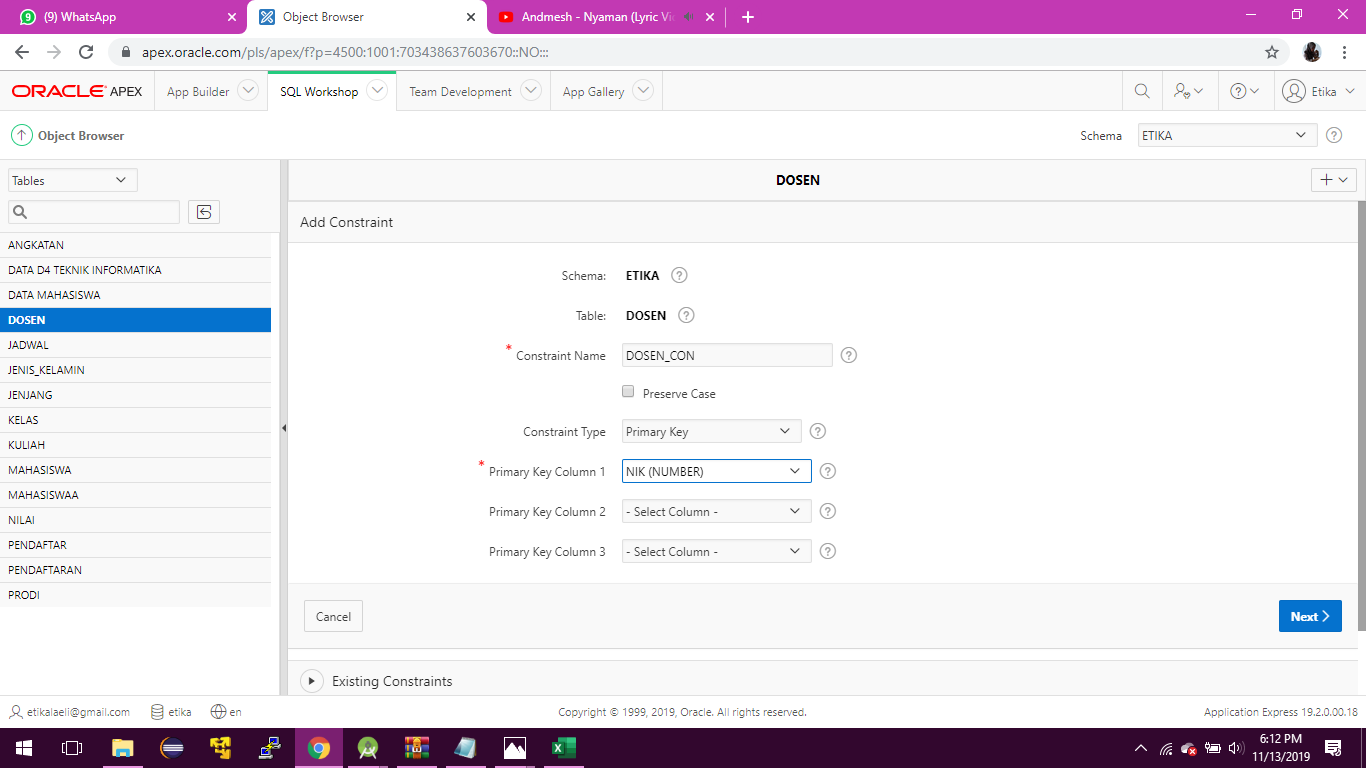
\includegraphics[scale=0.3]{figures/40.png}
    \caption{\textit{Tabel Dosen.}}
    \end{center}
    \label{gambar}
    \end{figure}

\begin{figure}
\item[25.]Pilih Tabel Kuliah, Clik Constrains, create Jadikan Kode Sebagai Primary Key, Lalu Next. 
    \begin{center}
    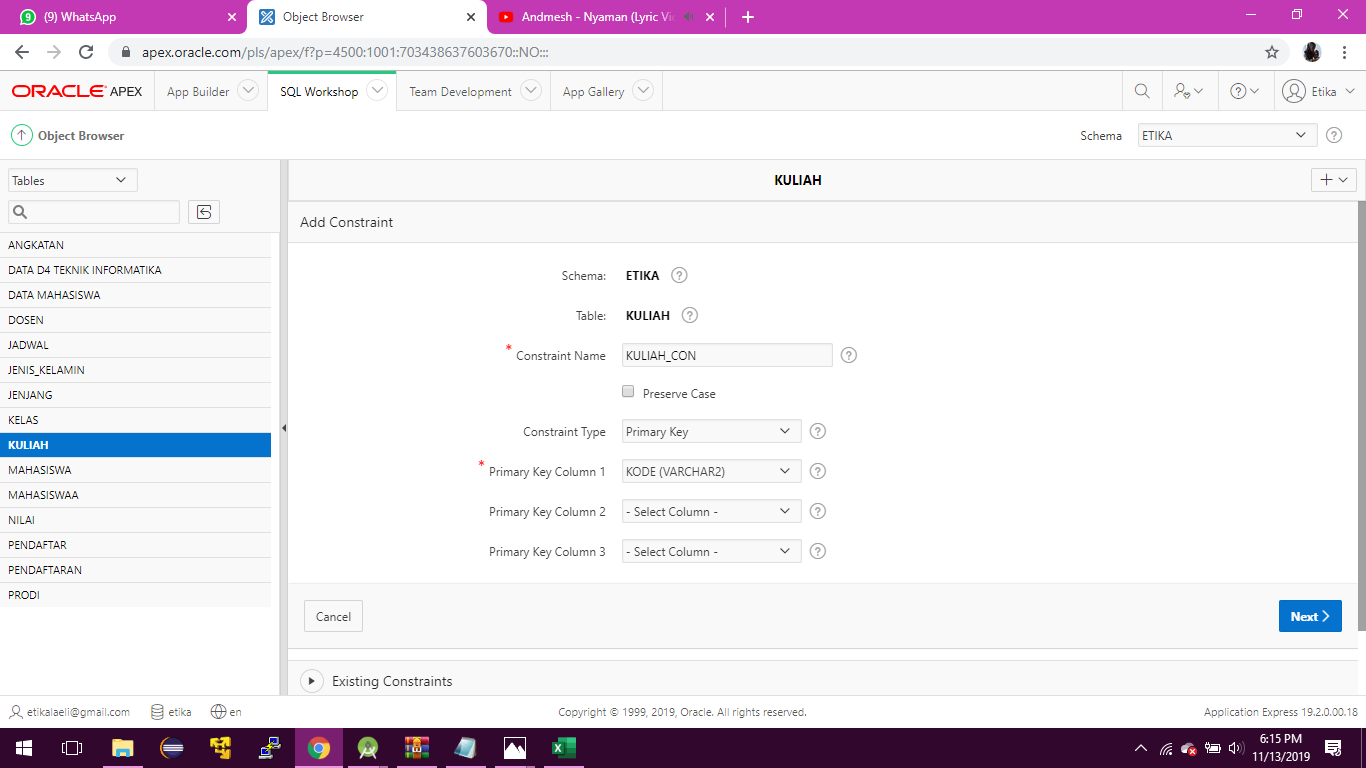
\includegraphics[scale=0.3]{figures/43.png}
    \caption{\textit{Tabel Kuliah.}}
    \end{center}
    \label{gambar}
    \end{figure}

\begin{figure}
\item[26.]Selanjutnya pilih tabel jadwal,Clik Constrains, create pilih foreign key jadikan kode di tabel sebalah kiri dengan table name kuliah dan table colum kode sebelah kiri.
    \begin{center}
    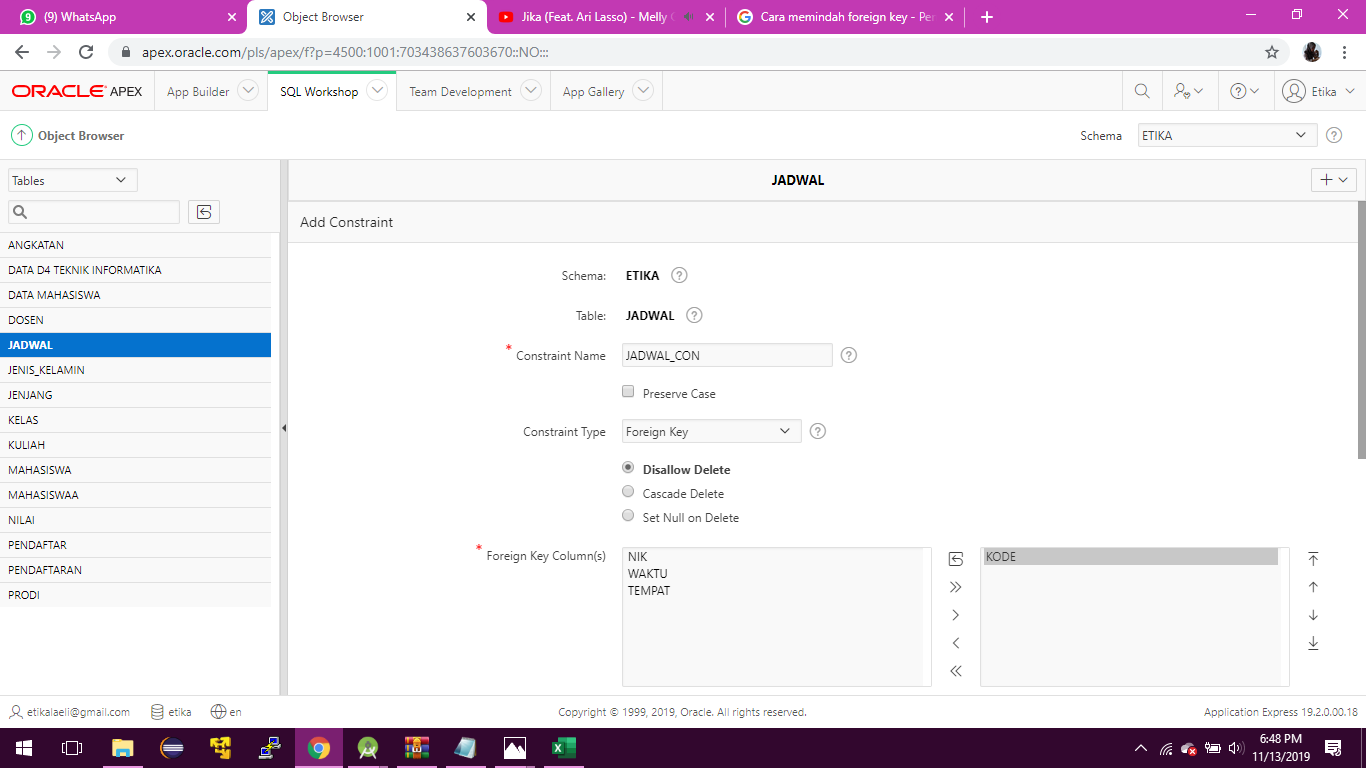
\includegraphics[scale=0.3]{figures/48.png}
    \caption{\textit{Tabel Jadwal.}}
    \end{center}
    \label{gambar}
    \end{figure}
    
\begin{figure}
\item[27.]Selanjutnya pilih tabel jadwal,Clik Constrains, create pilih foreign key jadikan kode di tabel sebalah kiri dengan table name kuliah dan table colum kode sebelah kiri.    
    \begin{center}
    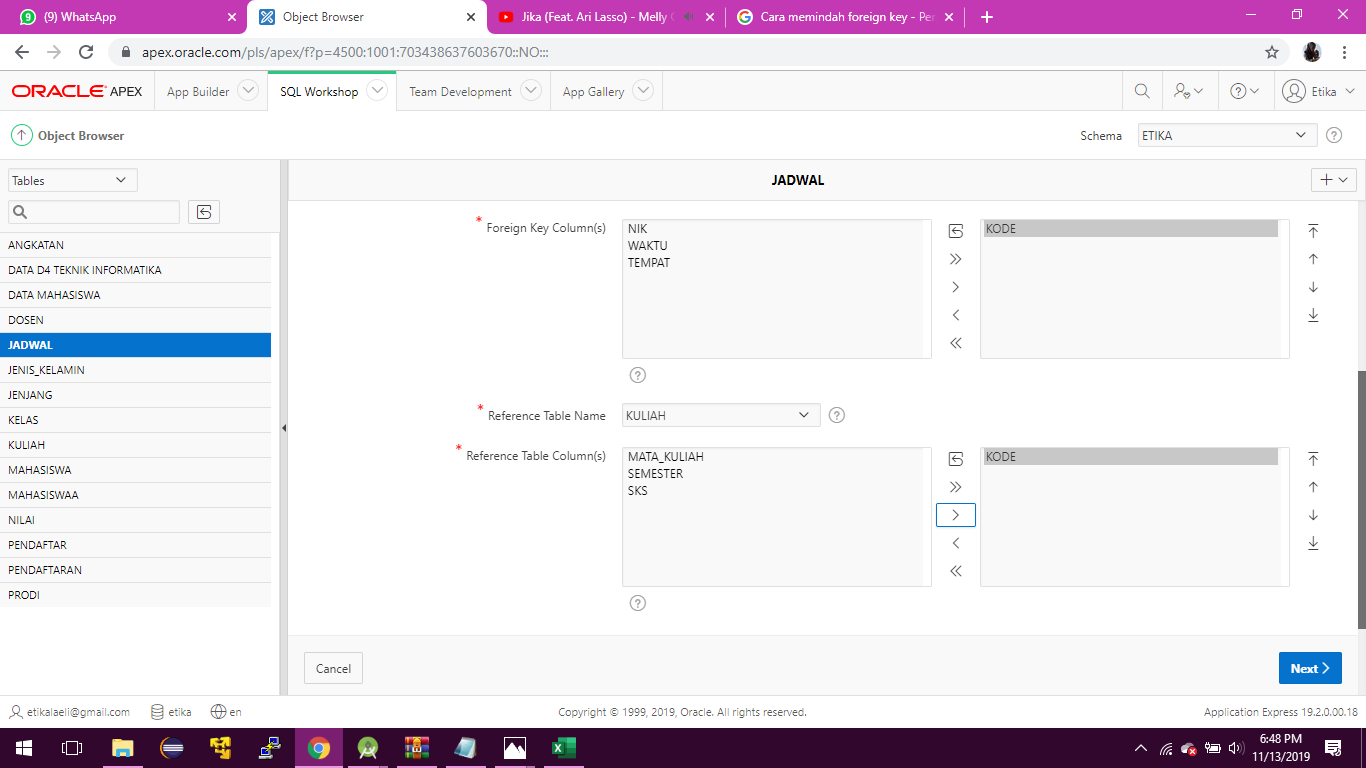
\includegraphics[scale=0.3]{figures/49.png}
    \caption{\textit{Table name Kuliah.}}
    \end{center}
    \label{gambar}
    \end{figure}

\begin{figure}
\item[28.] Selanjutnya pilih tabel Nilai,Clik Constrains, create pilih foreign key jadikan kode di tabel sebalah kiri dengan table name kuliah dan table colum kode sebelah kiri.
    \begin{center}
    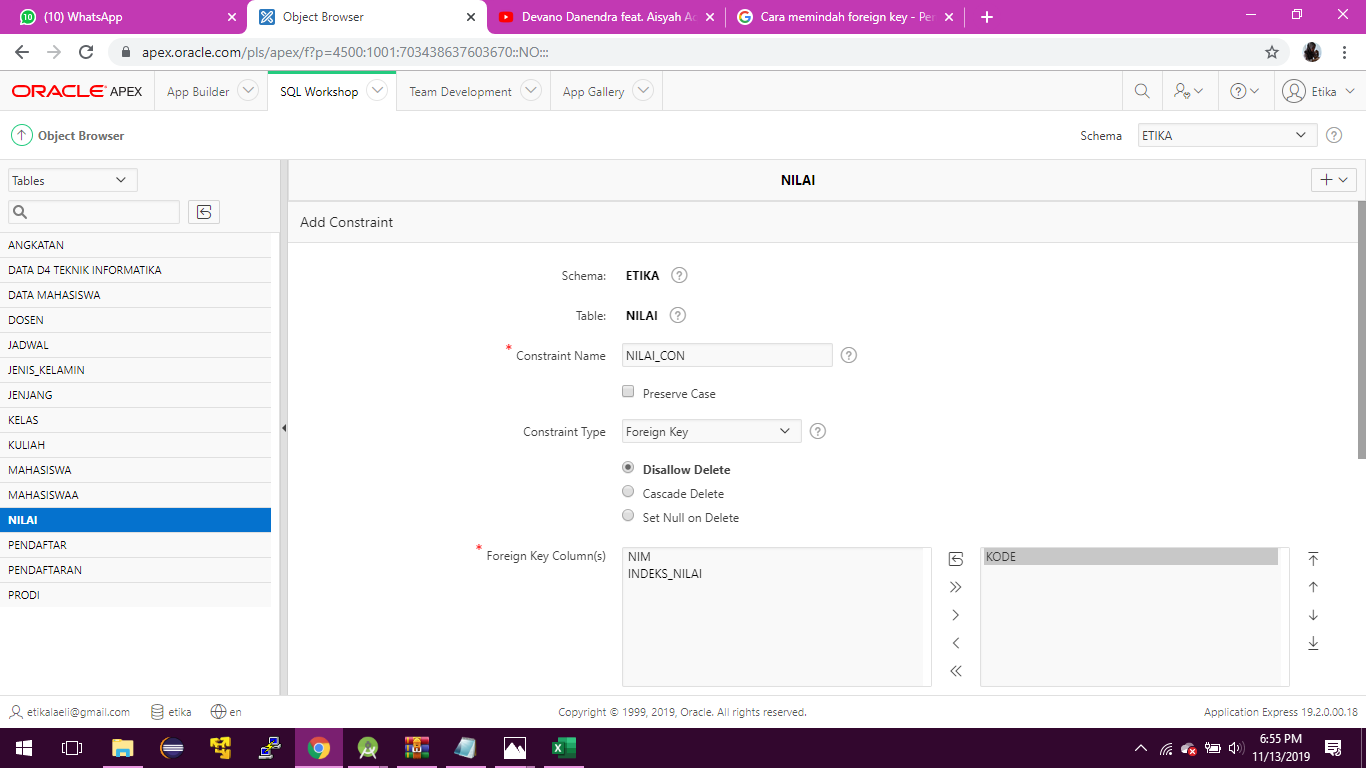
\includegraphics[scale=0.3]{figures/51.png}
    \caption{\textit{Tabel Nilai.}}
    \end{center}
    \label{gambar}
    \end{figure}

\begin{figure}
\item[29.] Selanjutnya pilih tabel Nilai,Clik Constrains, create pilih foreign key jadikan kode di tabel sebalah kiri dengan table name kuliah dan table colum kode sebelah kiri.    
    \begin{center}
    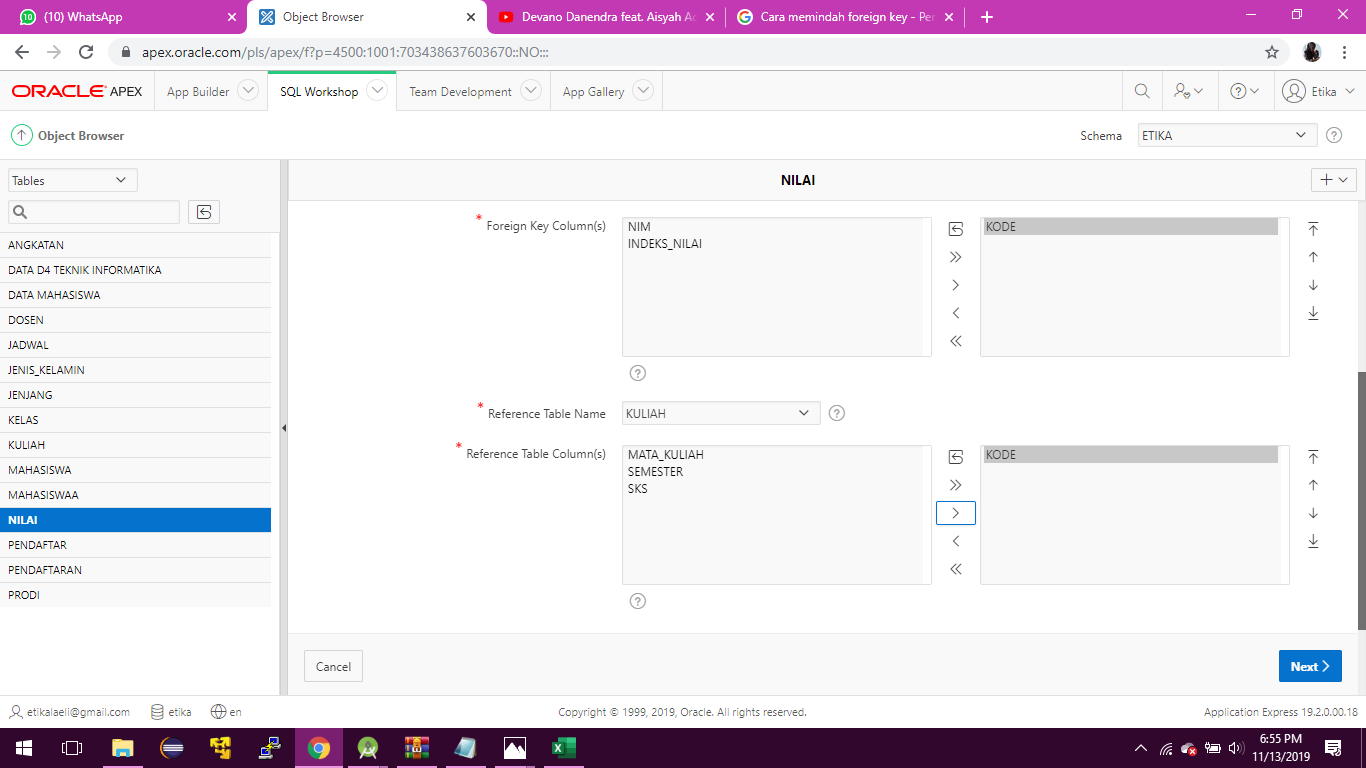
\includegraphics[scale=0.3]{figures/52.png}
    \caption{\textit{Table name kuliah.}}
    \end{center}
    \label{gambar}
    \end{figure}

\begin{figure}
\item[30.] Setelah itu buat nama aplikasi nya terlebih dahulu.
    \begin{center}
    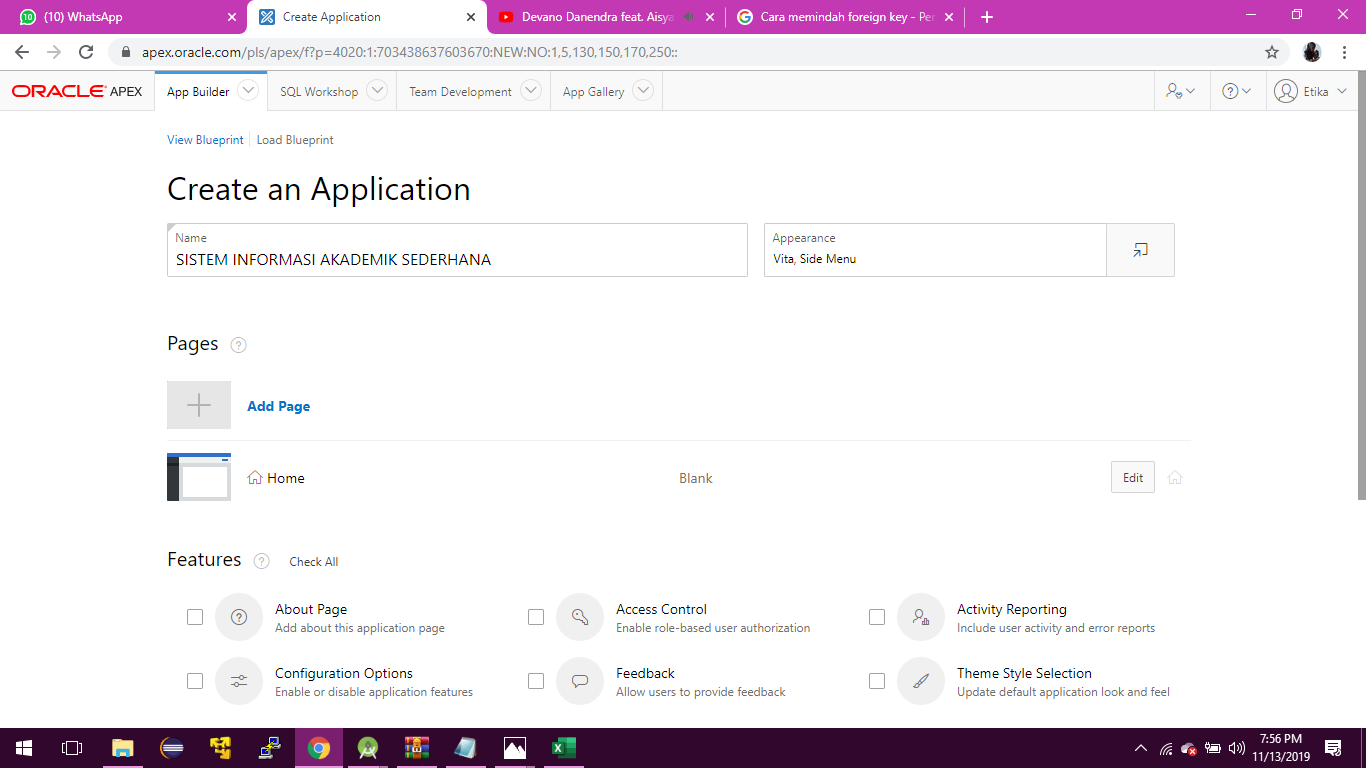
\includegraphics[scale=0.3]{figures/56.png}
    \caption{\textit{Nama Aplikasi.}}
    \end{center}
    \label{gambar}
    \end{figure} 
   
\begin{figure}   
\item[31.] Setelah itu pilih add page lalu pilih interactive report.
    \begin{center}
    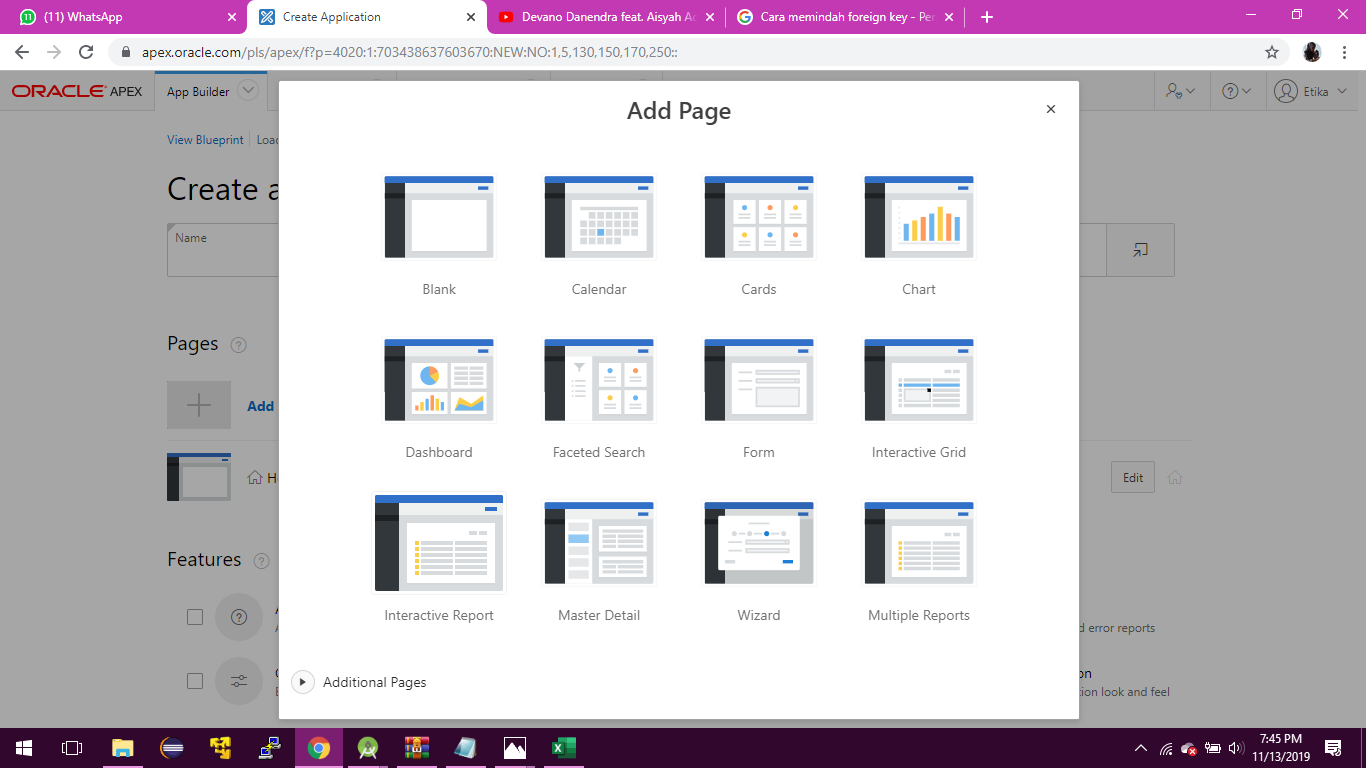
\includegraphics[scale=0.3]{figures/55.png}
    \caption{\textit{Add Page.}}
    \end{center}
    \label{gambar}
    \end{figure} 
     
\begin{figure}
\item[32.] Berinama tabel Mahasiswaa seperti gambar dibawah ini. Selanjutnya Create Application.
    \begin{center}
    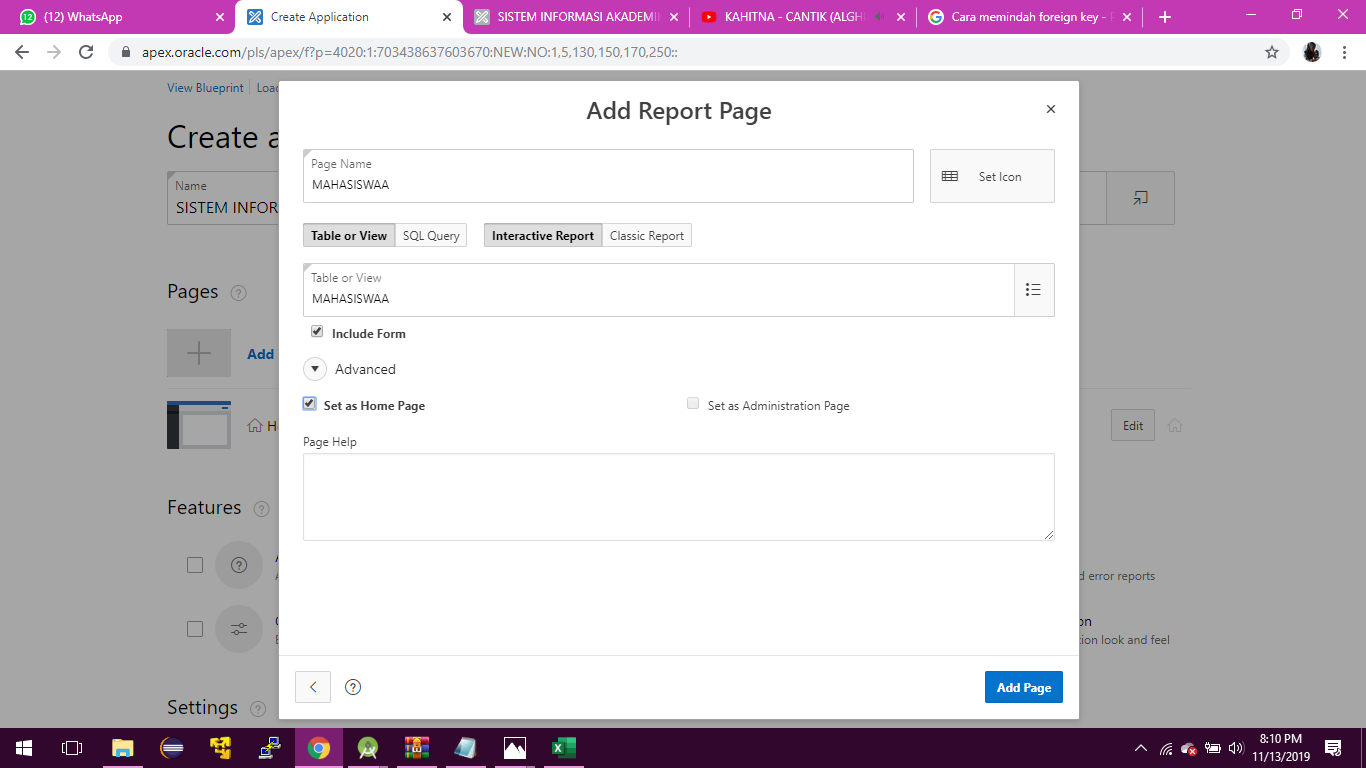
\includegraphics[scale=0.3]{figures/60.png}
    \caption{\textit{Add Page Tabel Mahasiswaa.}}
    \end{center}
    \label{gambar}
    \end{figure}

\begin{figure}
\item[33.] Berinama tabel Dosen seperti gambar dibawah ini. Selanjutnya Create Application.    
    \begin{center}
    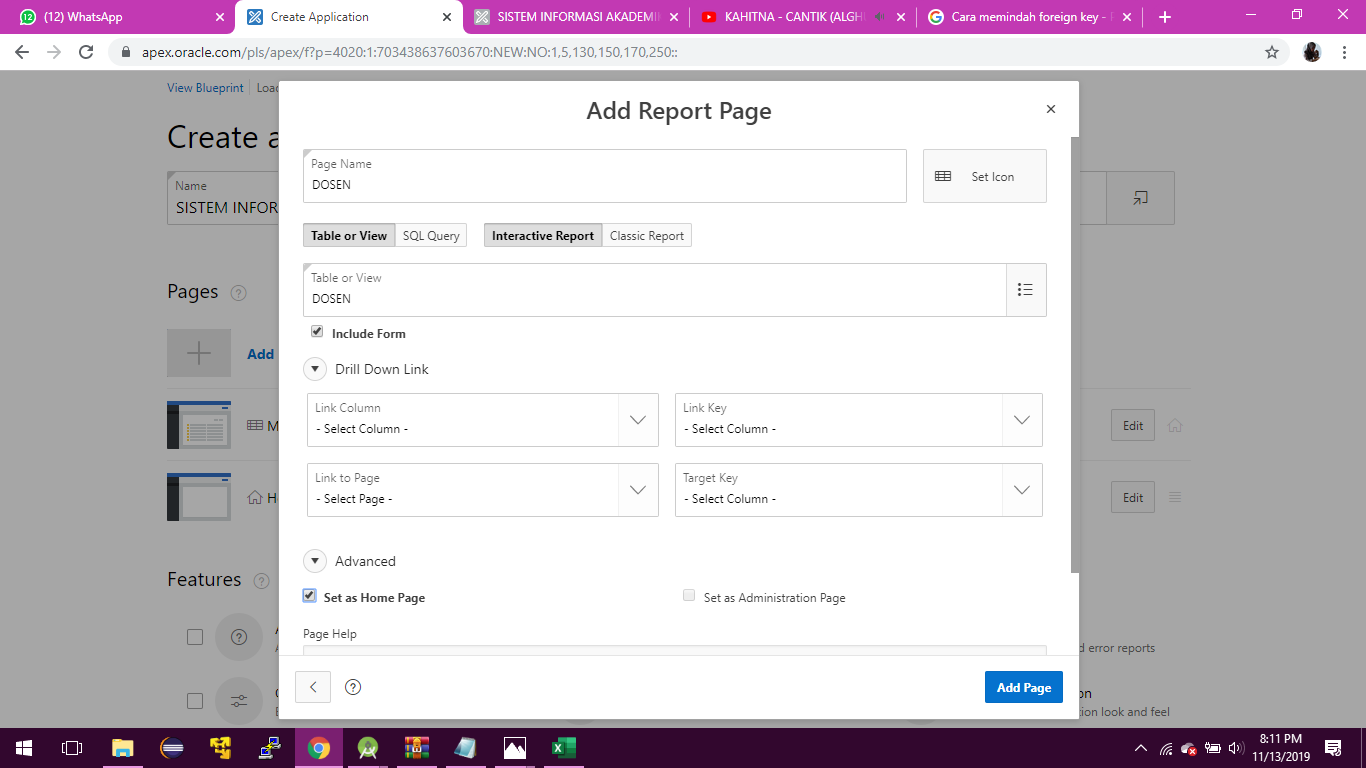
\includegraphics[scale=0.3]{figures/61.png}
    \caption{\textit{Add Page Tabel Dosen.}}
    \end{center}
    \label{gambar}
    \end{figure} 

\begin{figure}
\item[34.] Berinama tabel Kuliah seperti gambar dibawah ini. Selanjutnya Create Application.    
    \begin{center}
    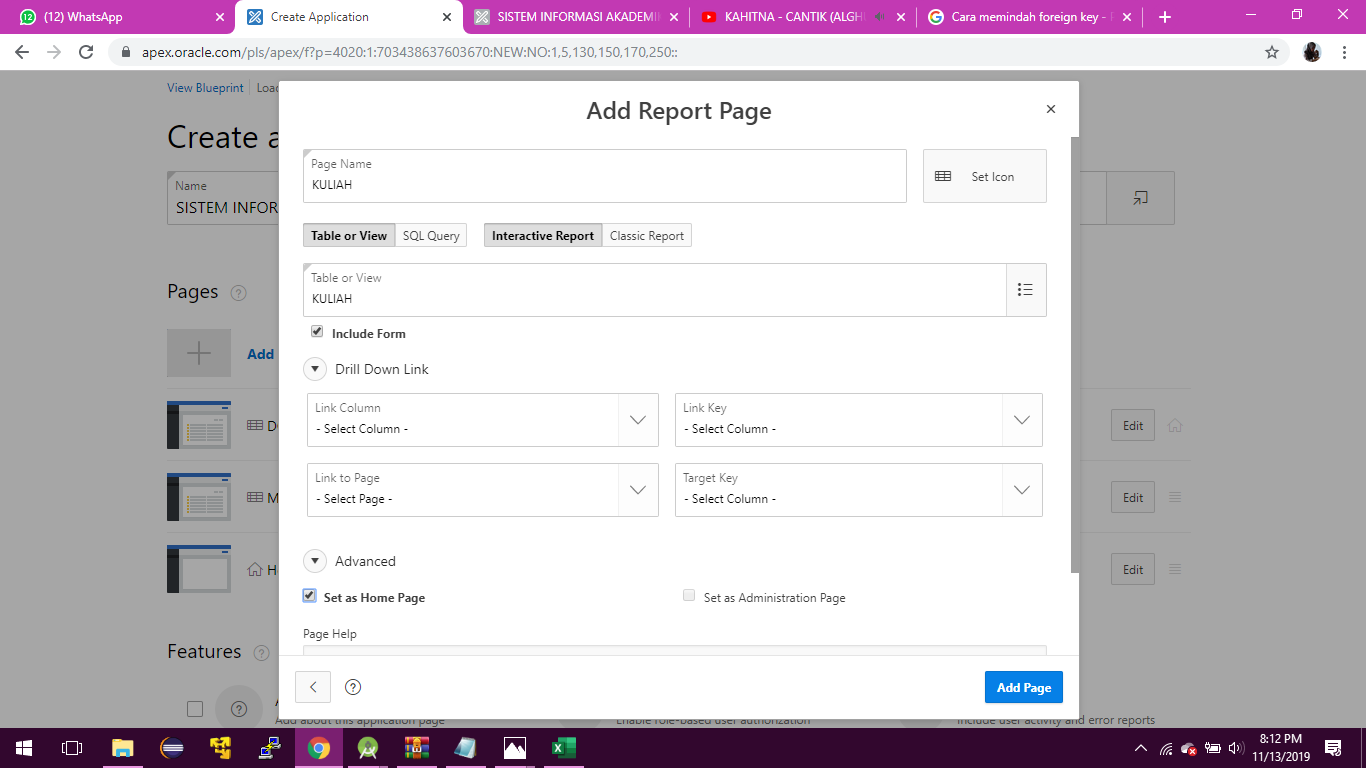
\includegraphics[scale=0.3]{figures/62.png}
    \caption{\textit{Add Page Tabel Kuliah.}}
    \end{center}
    \label{gambar}
    \end{figure}    

\begin{figure}
\item[35.] Berinama tabel Nilai seperti gambar dibawah ini. Selanjutnya Create Application.	
	\begin{center}
    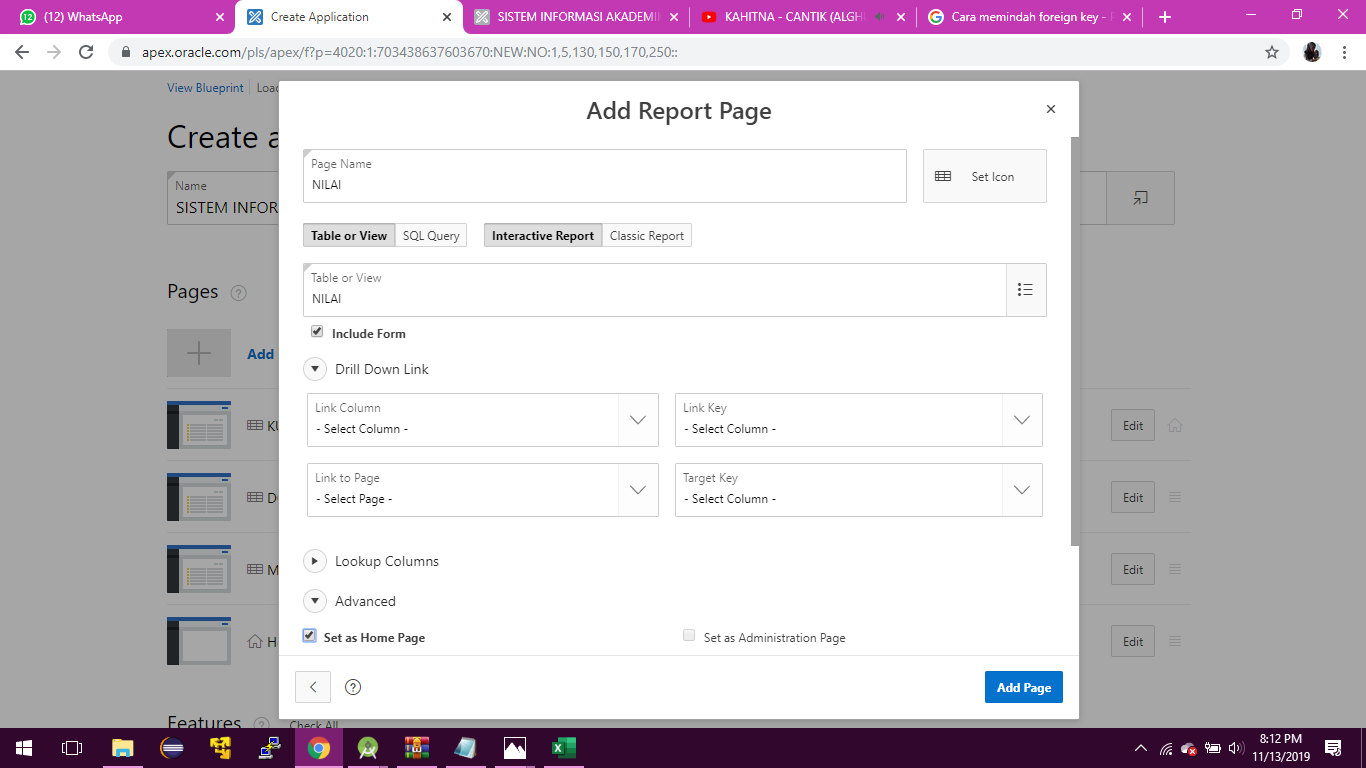
\includegraphics[scale=0.3]{figures/63.png}
    \caption{\textit{Add Page Tabel Nilai.}}
    \end{center}
    \label{gambar}
    \end{figure}

\begin{figure}
\item[36.] Berinama tabel Jadwal seperti gambar dibawah ini.Selanjutnya Create Application.    
    \begin{center}
    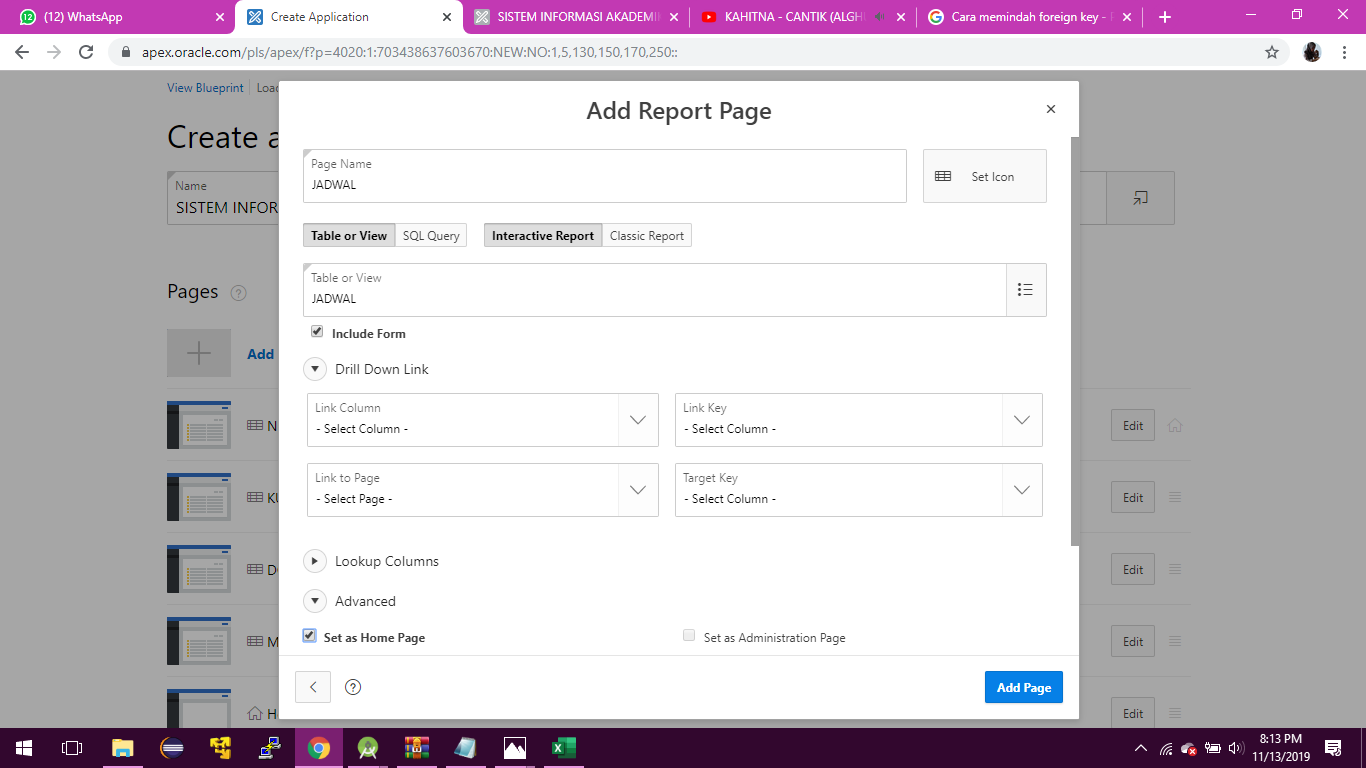
\includegraphics[scale=0.3]{figures/64.png}
    \caption{\textit{Add Page Tabel Jadwal.}}
    \end{center}
    \label{gambar}
    \end{figure}    

\begin{figure}
\item[37.]Setelah create application, tunggu beberapa saat untuk proses pembuatan aplikasi.
    \begin{center}
    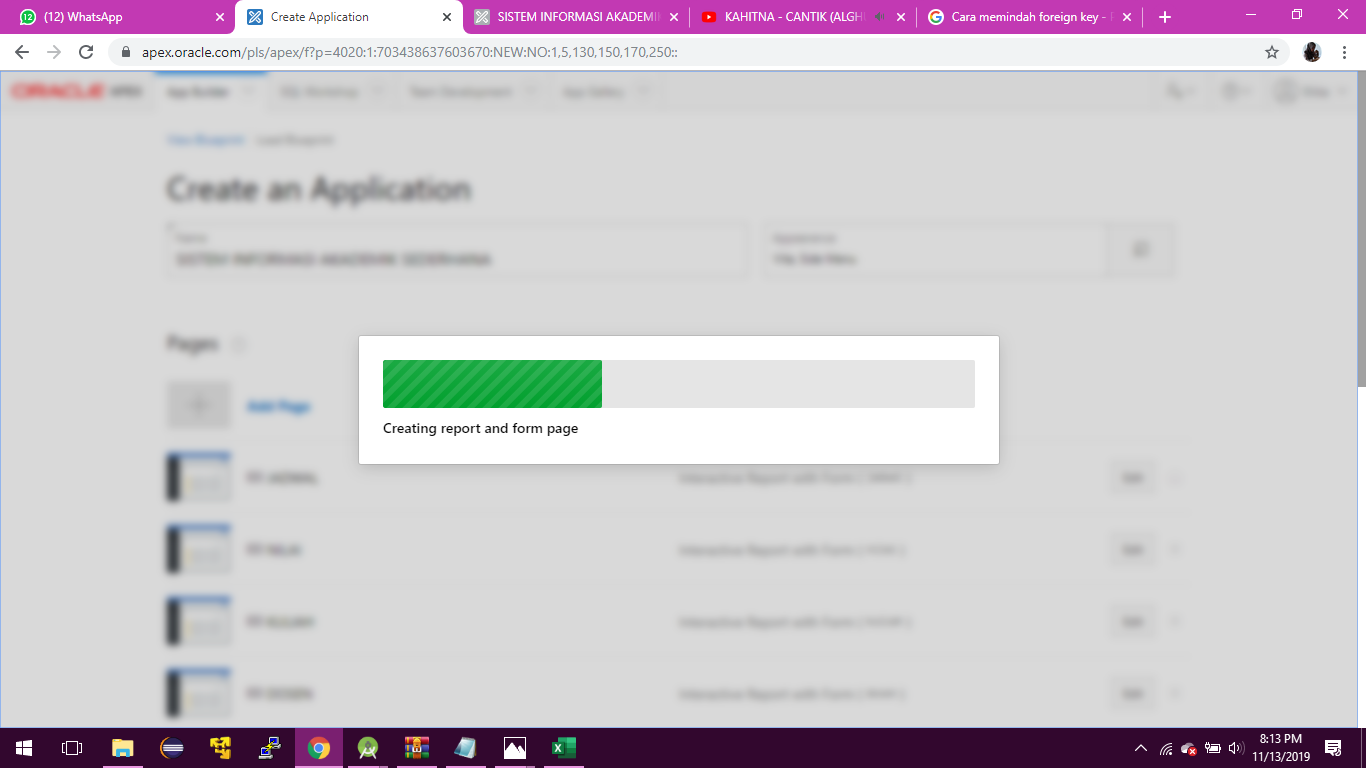
\includegraphics[scale=0.3]{figures/65.png}
    \caption{\textit{Loading.}}
    \end{center}
    \label{gambar}
    \end{figure}   

\begin{figure}
\item[38.]Selanjutnya kita Login dengan menggunakan email dan password kita.
    \begin{center}
    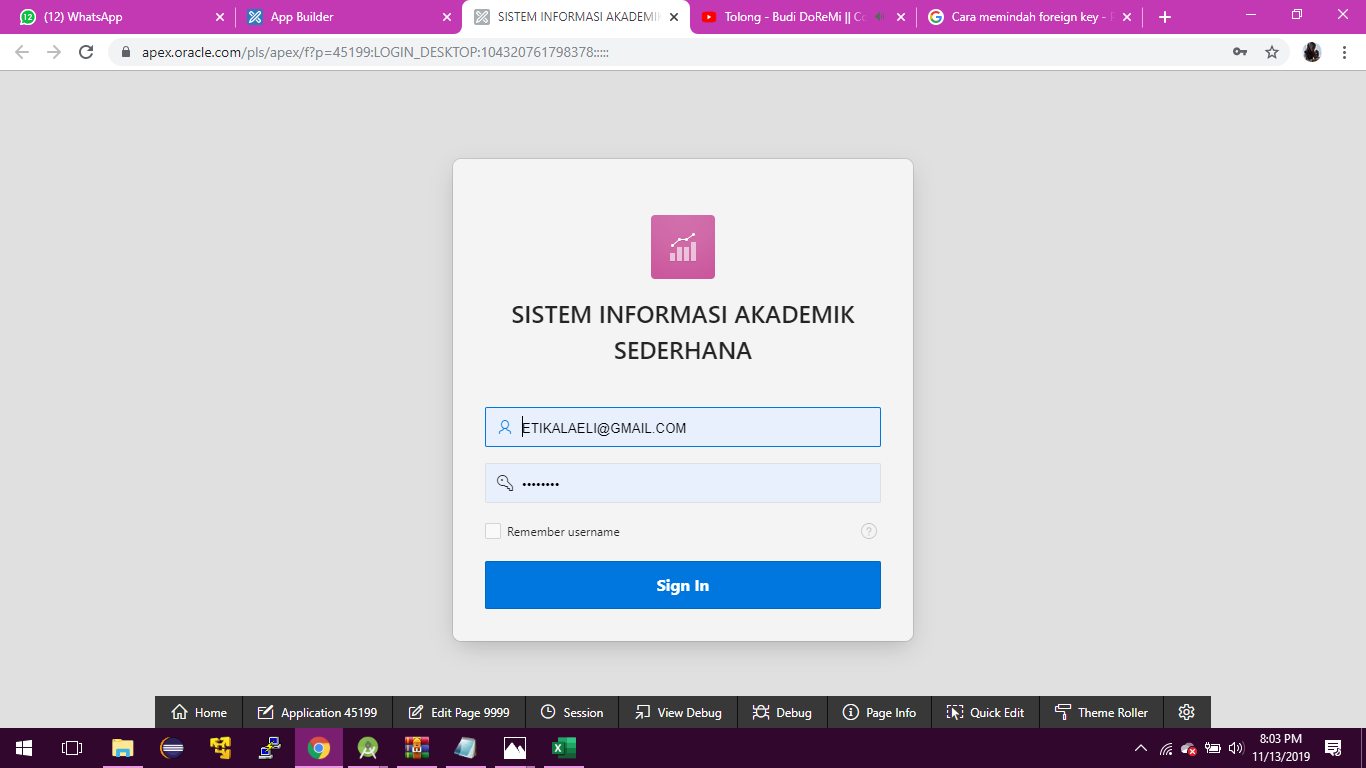
\includegraphics[scale=0.3]{figures/59.png}
    \caption{\textit{Login.}}
    \end{center}
    \label{gambar}
    \end{figure}   

\begin{figure}
\item[39.]Aplikasi Akademik Sederhana telah selesai dibuat.Disini kita bisa mengedit data atau mencari data yang diinginkan.
Username/email : etikalaeli@gmail.com
password : Etika17 (dedepan Etika Memakai pagar Menjadi pagarEtika17)
\href{https://apex.oracle.com/pls/apex/f?p=101498:7:107880375171823::NO:::}{LINK APLIKASI}
    \begin{center}
    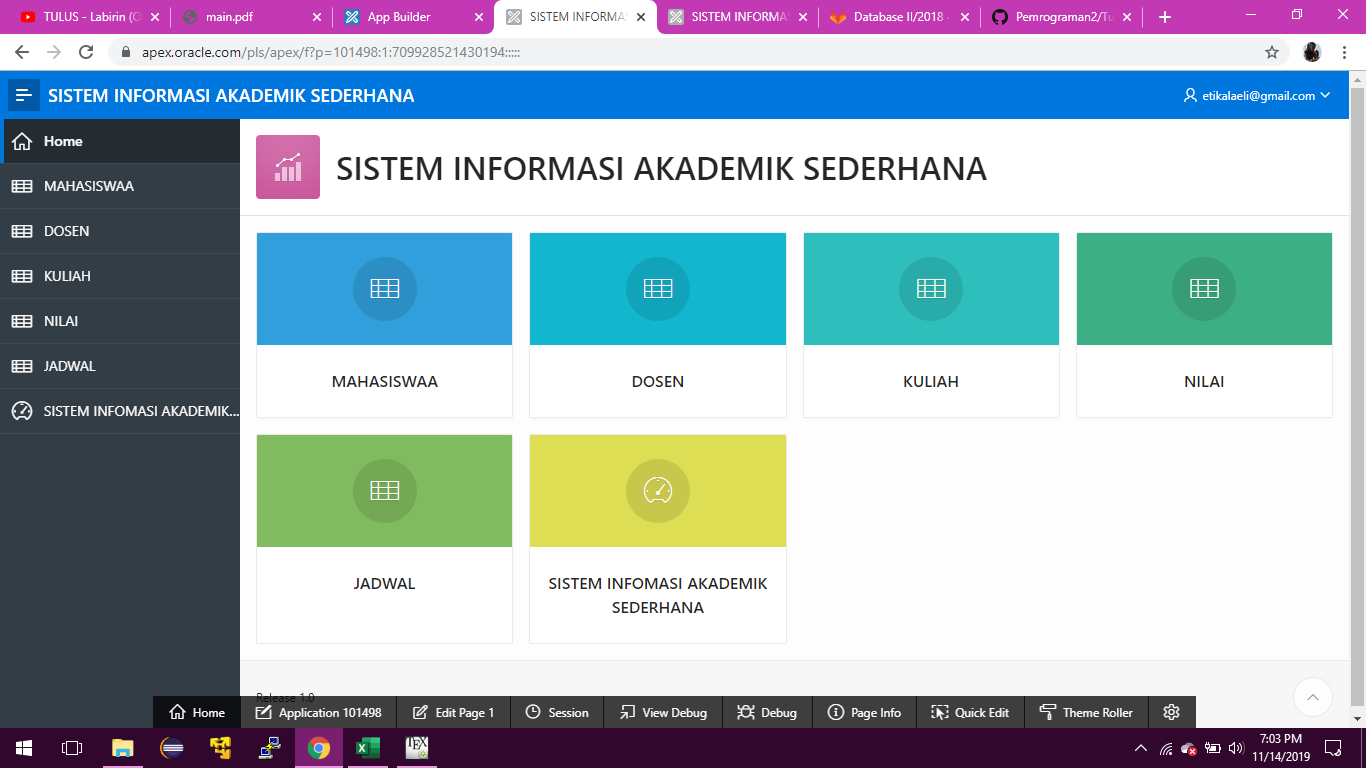
\includegraphics[scale=0.3]{figures/66.png}
    \caption{\textit{Home App Akademik Sederhana.}}
    \end{center}
    \label{gambar}
    \end{figure}   

\end{enumerate}
